\documentclass[conference]{IEEEtran}
\usepackage[T1]{fontenc}
\usepackage[utf8]{inputenc}
\IEEEoverridecommandlockouts
\usepackage{cite}
\usepackage{amsmath,amssymb,amsfonts}
\usepackage{graphicx}
\usepackage{textcomp}
\usepackage{xcolor}
\usepackage{hyperref}

\begin{document}

\title{FedBNR: A Fully Global Federated Gaussian Process}

\author{
  \IEEEauthorblockN{Risky Messages}
  \IEEEauthorblockA{
    Thus, even if we can learn the hyperparameters in a FL fashion without privacy leakage, we have to share X c / $\Phi$ c to calculate K and k ( x $\star$ , X ) .\\
  }
  \and
  \IEEEauthorblockN{Variance Adversarial Attack}
  \IEEEauthorblockA{
  }
  \and
  \IEEEauthorblockN{FedBNR+DP: Sensitivities}
  \IEEEauthorblockA{
  }
  \and
  \IEEEauthorblockN{Appendix B: Experiment Details}
  \IEEEauthorblockA{
    Figure 6 shows the architecture of DNNs used in the real world regression experiments. For FedAvg, FedProx, and pFedGP, we used the left DNN as their feature extractor. For our methods, we used the rightmost architecture in Fig. 2 with the same feature extractor f , a very small distribution shifter h (the right DNN in Fig. 6 ), and $\omega$ $\sim$ N ( 0 , I 5 ) .\\
  }
  \and
  \IEEEauthorblockN{Appendix C: Additional Results}
  \IEEEauthorblockA{
  }
  \and
  \IEEEauthorblockN{Generalization Setting}
  \IEEEauthorblockA{
  }
  \and
  \IEEEauthorblockN{Differential Privacy}
  \IEEEauthorblockA{
  }
  \and
  \IEEEauthorblockN{Personalization Setting}
  \IEEEauthorblockA{
  }
  \and
  \IEEEauthorblockN{Appendix D: Unifying Random Kernel}
  \IEEEauthorblockA{
  }
  \and
  \IEEEauthorblockN{Approximate Deep Stationary Kernels}
  \IEEEauthorblockA{
    Theorem A.1 (Hoeffding's inequality). Suppose X 1 , $\cdot$ $\cdot$ $\cdot$ , X n are n independent random variables. Let $\bar{}$ X = $\sum$ n i =1 X i /n . If $\forall$ i $\in$\{ 1 , $\cdot$ $\cdot$ $\cdot$ , n \} , Pr( X i $\in$ [ a i , b i ]) = 1 almost surely, then $\forall$ t > 0\\
  }
  \and
  \IEEEauthorblockN{Approximate Non-stationary Kernels Without DNN}
  \IEEEauthorblockA{
    ligence and statistics , pp. 370--378. PMLR. Wilson, A., \& Nickisch, H. (2015). Kernel interpolation for scalable structured Gaussian processes (kiss-gp).\\
    In: International conference on machine learning , pp. 1775--1784. PMLR. Xia, X., Sivonxay, E., Helms, B. A., Blau, S. M., \& Chan, E. M. (2023). Accelerating the design of multishell\\
  }
  \and
  \IEEEauthorblockN{Pascal Poupart}
  \IEEEauthorblockA{
    3 Noah's Ark Lab, Huawei Technologies, Shenzhen, China\\
    xi.chen11@mcgill.ca
  }
  \and
  \IEEEauthorblockN{4 MiniMax, Beijing, China}
  \IEEEauthorblockA{
  }
}
\maketitle

\begin{abstract}
Uncertainty estimation plays a key role in many practical areas such as simulation and parameter optimization. Gaussian process (GP) is one popular model that provides natu rally well-calibrated uncertainty estimates. However, it is challenging to learn a global GP posterior under the federated learning (FL) framework. In FL, clients' private data should not be shared, but merging local kernels directly leads to privacy leakage. Previous works that consider federated GPs avoid it and focus on the personalized setting. This sacrifices information from other clients that can be exploited to benefit generalization. We present Federated Bayesian Neural Regression (FedBNR) that learns a global federated GP while respecting clients' privacy. We incorporate deep kernel learning and random features by defining a unifying random kernel (URK). URK enables a principled approach of learning a global posterior as if all client data is centralized. Experiments conducted on real world regression datasets show statistically significant improvements.
\end{abstract}
\begin{IEEEkeywords}
Federated learning, Gaussian process, Random feature, Bayesian method
\end{IEEEkeywords}
\section{FedBNR: A Fully Global Federated Gaussian Process}
Haolin Yu 1,2 $\cdot$ Kaiyang Guo 3 $\cdot$ Mahdi Karami 1 $\cdot$ Guojun Zhang 4 $\cdot$ Hongliang Li 3 $\cdot$ Xi Chen 3 $\cdot$ Pascal Poupart 1,2

Machine Learning (2026) 115:72 https://doi.org/10.1007/s10994-025-06936-5

\section{Introduction}
Uncertainty estimation has been an indispensable part of many practical areas. For example, in simulations widely used for the development of aircraft, trains, and vehicles (Danquah et al., 2020 ) and the testing of safeguarding autonomous vehicles (Riedmaier et al., 2020 ), uncertainty estimation is needed to assess the uncertainty inherent in any simulation model (Riedmaier et al., 2021 ). Researchers have also been using Bayesian optimization to speed up material design with nanoparticles (Xia et al., 2023 ; Iyer et al., 2020 , 2019 ), where uncertainty estimation is used to balance exploitation and exploration. In machine-assisted decision making (Begoli et al., 2019 ), it provides the trust needed to inform decisions.

Machine Learning (2026) 115:72

Gaussian process (GP) has been an especially popular model that provides uncertain estimates (Verrelst et al., 2013 ; Li et al., 2021 ). GPs with deep kernel learning (Wilson et al., 2016a , 2016b ) provide a good balance between expressiveness and simplicity to represent model uncertainty. At one end of the spectrum, most traditional models such as traditional neural networks do not capture any uncertainty, but are simple and scalable. At the other end of the spectrum, Bayesian neural networks express a full distribution over all weights of neural networks, but exact inference tends to be infeasible. In between, a GP with a deep kernel consists of a deep neural feature extractor with a distribution over the last layer that facilitates exact inference. Since the last layer is the most important for prediction, representing its uncertainty is often sufficient to capture most of the uncertainty of a model (Gawlikowski et al., 2022 ; Kristiadi et al., 2020 ).

However, extending GPs to the federated learning (FL) setting itself is challenging. In FL, we seek to train a model in a distributed way across several clients without any data leav ing the clients to preserve privacy. Several works have explored distributed GPs (Deisenroth \& Ng, 2015 ; Yin et al., 2020 ) and federated GPs (Achituve et al., 2021 ; Kontoudis \& Stil well, 2023 , 2024 ). While distributed GPs are designed to improve scalability, they pose an important privacy risk since sharing kernels either implies sharing data or sharing pairwise data similarity. In contrast, federated GPs including pFedGP (Achituve et al., 2021 ),DEC- apx-GP (Kontoudis \& Stilwell, 2023 ), and DEC-gapx-GP (Kontoudis \& Stilwell, 2024 ) share only the hyperparameters of kernels while learning local GP posteriors that are never shared. This personalized approach reduces privacy risks, but the local GPs do not benefit from other client information beyond the shared kernel hyperparameters. Thus, its accu racy suffers when generalization is desired or new clients come without training data. For example, a hospital that only collected chest X-rays of lung emphysema patients may also want their model to help diagnose rib fractures with the same type of input. However, per sonalization would prevent the model from generalizing to other ranges. Moreover, new clients with few training data cannot effectively train predictors with local GPs, even if they do not need generalization.

To address such challenges, we propose a new federated GP technique called Federated Bayesian Neural Regression (FedBNR) that learns a global federated GP. We first define a unifying random kernel (URK) which allows random feature approximation of both sta tionary and non-stationary kernels. FedBNR with URK avoids kernel sharing by working directly in the feature space and sharing scatter matrices, reducing privacy risks and decreas ing the computational complexity to linear in the amount of data. Since FedBNR maintains a global posterior, it makes full use of different clients' information, and performs better for generalization and new clients. The approach is demonstrated on real world regression data sets where we achieve statistically significant improvements over prior techniques both in terms of point and uncertainty estimation. We further extend our algorithm with differential privacy to provide formal privacy guarantees. The main contributions are:

$\bullet$ New random feature approximations of non-stationary kernels enabled by URK, and their concentration guarantees. $\bullet$ A new federated GP technique FedBNR, which achieves better generalization perfor mance in both accuracy and uncertainty calibration due to its global posterior.

\section{Page 2 of 36}
Machine Learning (2026) 115:72

The paper is structured as follows. In Sect. 2 , we review essential background knowledge of GP, FL, and related works. In Sect. 3 , we introduce URK and its theoretical guarantees, pro pose FedBNR based on URK, and extend FedBNR with differential privacy (DP). Sect. 4 details synthetic and real-world experiments. Finally, Sect. 5 concludes the work.

\section{Background}
Notation. We use the following notation throughout the paper. X , X $'$ $\in$ R p $\times$ n , x , x $'$ $\in$ R p are input matrices or vectors. n is the number of data points and p is the number of features. y $\in$ R n is the target vector. x $*$ , y $*$ indicate vectors that have not been seen by the models. $\sigma$ $\in$ R + is the standard deviation of the additive Gaussian noise in the models we men tion later. I is the identity matrix and 0 is the zero vector. Their dimensions can be inferred from the context. $\phi$ : R p $\rightarrow$ R d denotes a d dimensional basis function, and $\Phi$ = $\phi$ ( X ) denotes the corresponding features of X . k : R p $\times$ R p $\rightarrow$ R denotes a kernel function, and K = k ( X , X ) is the corresponding kernel Gram matrix. w $\in$ R d are the weights of the linear layer in a Bayesian linear regression model. $\lambda$ $\in$ R + is the prior standard deviation on w . E [ $\cdot$ ] , Cov ( $\cdot$ , $\cdot$ ) , and Tr ( $\cdot$ ) are the expectation, covariance, and trace function. Any symbol with a c subscript is a local version of the original symbol, held by client c .

\section{Gaussian Process and Random Fourier Feature}
A GP can be viewed as an infinite dimensional Gaussian distribution over function objects f ( $\cdot$ ) . If restricted to a finite set of points of interest X on the support, a GP becomes a multi-dimensional Gaussian distribution f ( X ) , providing distributional information at these places. Formally, GP regression with additive Gaussian noise is established as y = f ( x ) + $\epsilon$ , where $\epsilon$ $\sim$N (0 , $\sigma$ 2 ) . After a prior over f ( $\cdot$ ) is specified, the likelihood, posterior, and prediction can be computed as follows:

Prior: f ( $\cdot$ ) $\sim$GP ( 0 , k ( $\cdot$ , $\cdot$ )) (1)

Likelihood: ( y | X , f ( $\cdot$ )) $\sim$N ( f ( X ) , $\sigma$ 2 I ) (2)

Posterior: ( f ( $\cdot$ ) | X , y ) $\sim$GP ( $\bar{}$ m ( $\cdot$ ) , k $'$ ( $\cdot$ , $\cdot$ )) , where (3)

$\bar{}$ m ( $\cdot$ ) = k ( $\cdot$ , X )( K + $\sigma$ 2 I ) - 1 y , (4)

k $'$ ( $\cdot$ , $\cdot$ ) = k ( $\cdot$ , $\cdot$ ) - k ( $\cdot$ , X )( K + $\sigma$ 2 I ) - 1 k ( X , $\cdot$ ) (5)

Prediction: ( y $*$ | x $*$ , X , y ) $\sim$N ( $\bar{}$ m ( x $*$ ) , $\sigma$ 2 + k $'$ ( x $*$ , x $*$ )) (6)

The runtime complexity of GP is O ( n 3 ) due to K - 1 . Thus in practice, full GPs are often infeasible, and approximations are needed for scalability. The performance of GP models highly depends on the kernel function k ( $\cdot$ , $\cdot$ ) , and hyperparameters of this function can be learned by maximizing log Pr GP ( y | X ) = - y $^\top$ ( K + $\sigma$ 2 I ) - 1 y - log | K + $\sigma$ 2 I | .

Page 3 of 36 72

Machine Learning (2026) 115:72

A valid kernel function is any positive definite function and can always be decomposed into the inner product of some basis functions k ( x , x $'$ ) = $\phi$ ( x ) $^\top$ $\phi$ ( x $'$ ) (Cuturi, 2009 ). An important advantage of working in the function space (i.e., with kernels) is that kernel func tions can correspond to infinite features (i.e., the corresponding $\phi$ ( x ) must map x to infi nitely many linearly independent features) without paying a price in complexity. Popular kernels, such as the Gaussian kernel k ( x , x $'$ ) = exp( -|| x - x $'$ || 2 / 2 $\gamma$ 2 ) ( $\gamma$ $\in$ R + is a kernel hyperparameter), tend to induce infinite dimensional features, providing significant model capacity.

If the kernel has finite features (i.e. $\exists$ $\phi$ ( x ) that maps x into finitely many features), a GP degenerates into Bayesian linear regression (BLR) in the feature space with parametrized model f ( $\cdot$ ) = w $^\top$ $\phi$ ( $\cdot$ ) . Given a prior over w , the likelihood, posterior, and prediction are:

Prior: w $\sim$N ( 0 , $\lambda$ 2 I ) (7)

\section{Likelihood: ( y | X , w ) $\sim$N ( w $^\top$ $\Phi$ , $\sigma$ 2 I ) (8)}
Posterior: ( w | X , y ) $\sim$N ($\bar{}$ w , A - 1 ) , where (9)

\section{$\bar{}$ w = $\sigma$ - 2 A - 1 $\Phi$ y and A = $\sigma$ - 2 $\Phi$$\Phi$ $^\top$ + $\lambda$ - 2 I (10)}
Prediction: ( y $*$ | x $*$ , X , y ) $\sim$N ( $\phi$ ( x $*$ )$\bar{}$ w , $\sigma$ 2 + $\phi$ ( x $*$ ) $^\top$ A - 1 $\phi$ ( x $*$ )) (11)

Recall $\phi$ ( X ) $\in$ R d . Then the complexity of BLR is O ( nd 2 + d 3 ) due to A - 1 . Hyperparameters of $\phi$ can be learned similarly by maximizing log Pr BLR ( y | X ) = - n log $\sigma$ 2 - log | $\lambda$ 2 I | - log | A | -|| y - $\Phi$ $\bar{}$ w || 2 - $\lambda$ - 2 $\bar{}$ w $^\top$ $\bar{}$ w . It is very important to note that Eqs. 6 and 11 are identical, with only the order of matrix multiplication changed, resulting in different complexity and model interpretation.

Random Fourier features (RFF) (Rahimi \& Recht, 2007 ) can be used to approximate infinite stationary kernels with finite features based on Bochner's theorem:

Theorem 2.1 (Bochner's theorem, e.g. (Rudin, 2017 )). A continuous stationary kernel k ( x , x $'$ ) = $\tilde{}$ k ( x - x $'$ ) = $\tilde{}$ k ( $\delta$ ) on R p is positive definite if and only if $\tilde{}$ k ( $\delta$ ) is the Fourier transform of a non-negative measure.

Above, $\delta$ = x - x $'$ and $\tilde{}$ k is the kernel k redefined in terms of one argument that is the difference of the inputs x - x $'$ . If the kernel is real-valued and properly scaled, its inverse Fourier transform p ( $\omega$ ) is also real-valued and is a proper probability distribution. Then a valid feature mapping is z $\omega$ ( x ) = (cos( $\omega$ $^\top$ x ) , sin( $\omega$ $^\top$ x )) , since

\section{$\tilde{}$ k ( $\delta$ ) =}
\textbackslash\{\}\textasciicircum{}\{\}

R p p ( $\omega$ ) cos( $\omega$ $^\top$ $\delta$ ) d $\omega$ = E $\omega$ [cos( $\omega$ $^\top$ $\delta$ )] = E $\omega$ [ z $\omega$ ( x ) $^\top$ z $\omega$ ( x $'$ )]

The true expectation is then approximated by the empirical mean of z $\omega$ ( x ) $^\top$ z $\omega$ ( x $'$ ) with multiple samples from p ( $\omega$ ) , which enables recovering an infinite kernel with a finite set of features and working directly in the feature space.

\section{Page 4 of 36}
Machine Learning (2026) 115:72

\section{Federated Learning v.s. Distributed Learning}
In federated learning (FL), there is always a collection of clients c $\in$ S that wish to col laborate, and each client holds their own data D c = ( X c , y c ) locally. We seek to train some machine learning model M $\theta$ on these client data, with parameters $\theta$ . Conventionally, we would centralize all the data D = $\cup$

c $\in$ S D c , and learn the model globally. This simple approach becomes infeasible if the clients cannot directly share their data due to privacy concerns. FL is designed to specifically tackle this problem. In typical scenarios, a trusted central server is allowed to receive and send perturbed matrices that only contain limited information about raw client data such as model parameters.

Although FL seems similar to distributed learning (DL) where tasks are also distributed to client workers to exploit extra computational resources, FL focuses on settings that are very different from typical DL settings and thus faces unique challenges that DL algorithms cannot handle. First, DL algorithms are usually deployed on clusters, where communication between nodes are fast and reliable, thus algorithms with huge message throughput, like aggregating local gradients at each iterative step, are practical and feasible. However, in the cross-device setting of FL, client nodes are often millions of mobile devices that are not reliable and possess only limited computational resources. In this case, it is crucial to reduce the communication cost, so FL algorithms are often expected to aggregate local models or information that have evolved for more than one step or epoch of gradient descents from the previous global consensus, and a line of works (Konečny et al., 2016 ; Sattler et al., 2019 ; Reisizadeh et al., 2020 ) are dedicated in improving the communication efficiency. This nature of clients further leads to data and system heterogeneity, since the server often, if not always, has no control over how data or computation resource is distributed. More importantly, FL algorithms focus on reducing privacy risks of clients, while it is not a con cern at all of DL algorithms. Hence, many DL algorithms send risky messages with which other entities can easily retrieve the raw data of clients. A review with more details can be found in Appendix A.

\section{Related Work}
Distributed and Federated GPs Closely related to our work is the literature on distributed and federated GPs. Distributed GPs (Deisenroth \& Ng, 2015 ; Yin et al., 2020 ) were initially proposed to improve scalability by partitioning the data into several machines since GPs that operate in the dual space scale cubically with the amount of data in the worst case. The product-of-experts framework has emerged as a popular technique to aggregate local GPs, including generalized product of experts (Cao \& Fleet, 2014 ) and robust Bayesian committee machines (Deisenroth \& Ng, 2015 ). Distributed optimization of hyperparam eters in GPs has also been explored using ADMM (Xie et al., 2019 ), statistical parameter matching (Yurochkin et al., 2019 ), or variational inference (Gal et al., 2014 ; Hoang et al., 2016 ). While those techniques do not ensure data privacy, recent work about federated GPs reduce privacy risks while training in a distributed way. This includes pFedGP (Achituve et al., 2021 )and DEC-apx-GP (Kontoudis \& Stilwell, 2023 ) which optimize the hyperpa rameters of a global kernel using either FedAvg or decentralized proximal ADMM. DEC- gapx-GP (Kontoudis \& Stilwell, 2024 ) is an extension of DEC-apx-GP, which shares an additional dataset with all clients as extra training data. Note this violates the constraints of

Page 5 of 36 72

Machine Learning (2026) 115:72

FL, in the absence of a public dataset, since the additional dataset must consist of client's local data. These federated GP algorithms share only the hyperparameters of kernels, but learn local GP posteriors that are never shared. In another line of work, GPs have also been used to estimate correlations between clients in FL in order to actively select independent clients for aggregation (Tang et al., 2021 ). Our work differs from previous distributed and federated GPs by learning a global federated GP with better generalization performance.

Deep kernel learning and GP approximations There have been many works that commit ted to increasing the model capacity of GPs by incorporating deep neural networks (DNNs). Works of Hinton and Salakhutdinov ( 2007 ), Calandra et al. ( 2016 ) either pretrain a deep belief network or directly train it with a GP to extract first-step features before sending the data into the GP with conventional kernels. Wilson et al. ( 2016a , 2016b ) build their algo rithm on top of Wilson and Nickisch ( 2015 ), Wilson et al. ( 2015 ), Titsias ( 2009 ), Hensman et al. ( 2013 ), Nickson et al. ( 2015 ), extending this idea with approximations for scalability and stochastic variational inference for classification tasks. Then Tran et al. ( 2019 ) studies the variance estimations of deep kernel learning models and proposes to use Monte-Carlo Dropout (Gal \& Ghahramani, 2016 ) for better calibration. Ober et al. ( 2021 ) proposes to use Bayesian Neural Networks instead of deterministic DNNs to prevent over-fitting. Besides, Garnelo et al. ( 2018 ) designed a special architecture that makes it possible for DNNs to simulate GP behaviors. Damianou and Lawrence ( 2013 ) form GPs into a deep architecture that corresponds to a deep belief network based on GP mappings. To make GPs practi cal, one popular method is the inducing point approximation, where the joint GP prior of training points and inducing points are approximated (Quinonero-Candela \& Rasmussen, 2005 ). Variants includes SoD (Quinonero-Candela \& Rasmussen, 2005 ), SoR (Smola \& Bartlett, 2000 ), DTC (Seeger et al., 2003 ), FITC (Snelson \& Ghahramani, 2005 ), and PITC (Schwaighofer \& Tresp, 2002 ). Later, KISS-GP (Wilson \& Nickisch, 2015 ) gave another interpretation that inducing point approximations are equivalent to global GP interpolation, and it can exploit Kronecker structures (Saatçi, 2012 ). Another approximation method is random features (Rahimi \& Recht, 2007 ; Sinha \& Duchi, 2016 ; Oliva et al., 2016 ) that use randomized basis functions to approximate kernels. More information about scalable GPs can be found in this survey (Liu et al., 2020 ).

\section{Federated Learning of Global GPs}
Personalized federated learning (PFL) algorithms can learn fine-tuned local models for each client and can automatically handle preference distribution skew (Zhu et al., 2021 ) (i.e., Pr( y | X ) varies with clients). However, this comes at the cost of the generalization ability, especially when preference skew is not a concern and the clients want out-of-distribution generalization w.r.t. its training data. If a client is not capable of collecting enough data in the same range as their desired prediction, the accuracy of PFL local models could suf fer. For example, suppose the posterior of a GP with a stationary kernel is conditioned on local training data ( x 1 , $\cdot$ $\cdot$ $\cdot$ , x n c ) $\subset$ B c , an infinite compact set, and ( y 1 , $\cdot$ $\cdot$ $\cdot$ , y n c ) . Due to non-i.i.d. clients, it is common that other clients c $'$ have a different Pr( X ) in the form that B c $\cap$ B c $'$ / = B c $'$ . That is, training data of client c $'$ is considered out-of-range for client c . Suppose client c wants to generalize to the range of all clients' training data $\cup$ c $\in$ S B c . The prediction of data points from other clients' range x $'$ / $\in$ B c will gradually become the con

\section{Page 6 of 36}
Machine Learning (2026) 115:72

stant zero prior as x $'$ moves further from B c , regardless of what y $'$ really is. Thus, this gener alization error is unbounded. However, a global GP does exhibit a uniformly bounded error (Lederer et al., 2019 ), since its posterior is conditioned on all clients' data. It means all the clients, whether or not possessing training data, can benefit from others' information in FL.

With such motivation for learning global federated GPs, we derive our algorithm in the following sections. In Sect. 3.1 , we propose a random feature formulation URK, which is more flexible and compatible to deep learning as it can recover non-stationary kernels. It also provides more model capacity and thus better accuracy compared to plain deep learning without random features. Then, we detail our algorithm FedBNR in Sect. 3.2 , showing how a federated global posterior can be learned with URK. Finally, we extend FedBNR with DP in Sect. 3.3 , providing formal privacy guarantees (Fig. 1 ).

\section{GP Under Random Feature Maps}
URK Definition Recall that a kernel function can be rewritten as the inner product of some basis functions k ( x , x $'$ ) = $\phi$ ( x ) $^\top$ $\phi$ ( x $'$ ) . We propose the following kernel and random fea ture approximation.

Let $\omega$ $\in$ R d $'$ be any random variable or vector, and g : R d $'$ $\times$ R p -$\rightarrow$ R d be any function that extracts d features out of each input with random weights $\omega$ . We construct the random basis functions z as z $\omega$ ( x ) = g ( $\omega$ , x ) . We define the true underlying kernel and its approxi mation, the unifying random kernel (URK) as:

k ( x , x $'$ ) = E $\omega$ [ z $\omega$ ( x ) $^\top$ z $\omega$ ( x $'$ )] (12)

$\approx$ URK m $\omega$,g ( x , x $'$ ) :=

(

s m $\omega$ ( x ) $\sqrt{}$ m - 1

) $^\top$ (

s m $\omega$ ( x $'$ ) $\sqrt{}$ m - 1

)

= $\phi$ ( x ) $^\top$ $\phi$ ( x $'$ ) (13)

Fig. 1 FedBNR learns a global federated GP in two phases: kernel learning with federated optimization and last layer updating with exact Bayesian inference

Page 7 of 36 72

Machine Learning (2026) 115:72

where s m $\omega$ ( x ) is the concatenation of m samples of z $\omega$ ( x ) . Equation 12 is the true underlying kernel we construct. Equation 13 is the Monte-Carlo approximation of Eq. 12 , where the samples are the random features that URK produces. Furthermore, note

E $\omega$ [ z $\omega$ ( x ) $^\top$ z $\omega$ ( x $'$ )] = Tr ( Cov $\omega$ ( z $\omega$ ( x ) , z $\omega$ ( x $'$ ))) + E $\omega$ [ z $\omega$ ( x )] $^\top$ E $\omega$ [ z $\omega$ ( x $'$ )] (14)

Equation 14 follows from the definition of covariance (i.e., Cov ( A, B ) = E [ AB ] - E [ A ] E [ B ] , where A , B are random variables). Tr refers to the trace, which is needed for random vectors. It is a decomposition of the true underlying kernel, which provides an intuitive understand ing of the construction where URK mainly captures the covariance between different ran dom basis functions. This aligns with the purpose of the kernel function.

Examples and Theoretical Guarantees Since g is an arbitrary function, we can assign it any DNN with any architecture. We call it a kernel neural network (KNN) since its weights, $\theta$ , are essentially the kernel hyperparameters. It is trivial to map a deep kernel defined by k ( $\phi$ $\theta$ ( x ) , $\phi$ $\theta$ ( x $'$ )) , where k is any conventional stationary kernel and $\phi$ $\theta$ is any feature map ping function potentially represented by a deep neural network, into a URK construction:

\begin{figure}[htbp]
\centering
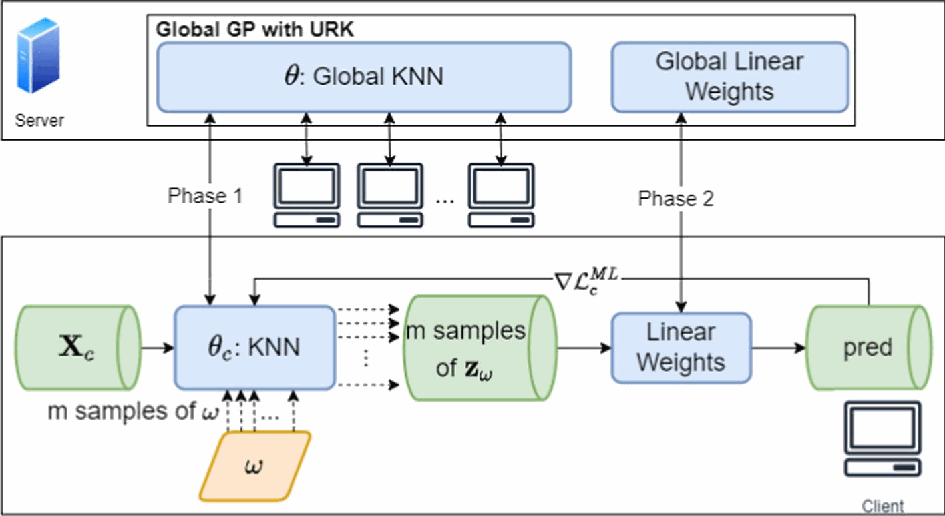
\includegraphics[width=\columnwidth]{fig_1_p7.png}
\caption{FedBNR learns a global federated GP in two phases: kernel learning with federated optimization and last layer updating with exact Bayesian inference}
\label{fig:1}
\end{figure}
\section{sin( $\omega$ $^\top$ $\phi$ $\theta$ ( x )) , cos( $\omega$ $^\top$ $\phi$ $\theta$ ( x )) ] $^\top$ (15)}
where p ( $\omega$ ) is the inverse Fourier transform of k . With m samples of $\omega$ , the error of approxi mating the true underlying kernel k ( x , x $'$ ) drops exponentially:

Theorem 3.1 $\forall$ x , x $'$ $\in$ R p , $\forall$ p ( $\omega$ ) being a proper distribution over R d $'$ , and g : R d $'$ $\times$ R p -$\rightarrow$ R d has the form of Eq. 15 . With m $\in$ Z + samples of $\omega$ , $\forall$ t > 0

Pr[ | URK m $\omega$,g ( x , x $'$ ) - k ( x , x $'$ ) | $\geq$ t ] $\leq$ 2 exp

(

- mt 2

)

URK can reconstruct not only conventional stationary kernels with a RFF mapping, but also non-stationary kernels beyond RFF's capability. We give two example constructions and their corresponding convergence properties below. Full proofs are in Appendix D.

The first example recovers a non-stationary kernel that induces infinite basis functions, like the Gaussian kernel.

Proposition 3.2 Let $\omega$ $\sim$ N ( 0 , I ) , g ( $\omega$, x ) = exp( $\omega$ $^\top$ x ) , then k ( x , x $'$ ) = lim m -$\rightarrow$ $\infty$ URK m $\omega$, g ( x , x $'$ ) is a non-stationary kernel with infinite features.

The following theorem bounds the error of URK approximation for the construction in Prop. 3.2 . Fenton-Wilkinson approximation (Fenton, 1960 ) is used to model the summation of log-normal distributions, and the error is bounded by the sum of two tail probabilities.

Theorem 3.3 Let $\omega$ and g have the form of Prop. 3.2 . Suppose x , x $'$ $\in$ R p satisfies || x || 2 2 $\leq$ a , || x $'$ || 2 2 $\leq$ a $'$ . With m $\in$ Z + samples of $\omega$ , $\forall$ t $\in$ ( 0 , exp( a + a $'$ ) / 2 )) , by Fenton- Wilkinson approximation,

\section{Page 8 of 36}
Machine Learning (2026) 115:72

$\sigma$ s := log

( exp ( a + a $'$ ) - 1

m + 1

)

, E := exp(( a + a $'$ ) / 2)

Pr[ | URK m $\omega$,g ( x , x $'$ ) - k ( x , x $'$ ) | $\geq$ t ] $\leq$ 1 - F ( 2 log( t + E ) - ( a + a $'$ ) + $\sigma$ 2 s 2 $\sigma$ s

)

+ F

( 2 log( E - t ) - ( a + a $'$ ) + $\sigma$ 2 s 2 $\sigma$ s

)

F is the cumulative probability distribution function of the standard normal distribution.

The second example recovers a popular non-stationary kernel, the polynomial kernel.

Proposition 3.4 Let $\tilde{}$c , $\tilde{}$n $\in$ R be hyperparameters of the polynomial kernel k ( x , x $'$ ) = ( x $^\top$ x $'$ + $\tilde{}$c ) $\tilde{}$n . Define $\tilde{}$ p = [ 1

2 , 1 2p , 1 2p , $\cdot$ $\cdot$ $\cdot$ , 1 2p ] $^\top$ $\in$ R p + 1 , $\omega$ $\sim$ Multi ( $\tilde{}$n , $\tilde{}$ p ) , the multinomial distribution. Define $\tilde{}$ x = [ $\sqrt{}$

2$\tilde{}$c , $\sqrt{}$ 2p x $^\top$ ] $^\top$ $\in$ R p + 1 , g ( $\omega$, x ) = exp( $\omega$ $^\top$ log $\tilde{}$ x ) , then k ( x , x $'$ ) = lim m -$\rightarrow$ $\infty$ URK m $\omega$, g ( x , x $'$ ) = ( x $^\top$ x $'$ + $\tilde{}$c ) $\tilde{}$n .

The following theorem bounds the error of URK approximation for the construction in Prop. 3.4 , with Hoeffding's inequality (Hoeffding, 1994 ) similarly to Thm. 3.1 .

Theorem 3.5 Let $\omega$ and g have the form of Prop. 3.4 . Suppose entries of x , x $'$ $\in$ R p + are bounded by [a, b]. With m $\in$ Z + samples of $\omega$ , $\forall$ t > 0 ,

v := max \{

$\sqrt{}$

2$\tilde{}$ c, $\sqrt{}$ 2 pb \} min \{ $\sqrt{}$

2$\tilde{}$ c, $\sqrt{}$ 2 pa \}

Pr[ | URK m $\omega$,g ( x , x $'$ ) - k ( x , x $'$ ) | $\geq$ t ] $\leq$ 2 exp

( - 2 mt 2

v 4$\tilde{}$ n

)

Without Randomness Note the deep features themselves already allow a valid BLR for mulation that is equivalent to a linear kernel. However, it is restricted to finite basis func tions as the same size of the second last layer and has the implicit assumption that the target is linear in the features. As the most basic kernel function, the linear kernel does not provide additional model capacity to the deep neural network. Previously, deep kernel learning algo rithms (Wilson et al., 2016a , 2016b ) apply the Gaussian kernel, which induces infinite basis functions, to deep features and show they effectively improve the model accuracy compared to using deep features only. The rationale is straightforward: adding extra basis functions to a model never worsens its training accuracy, and GPs are resilient to over-fitting. Adding randomness with the URK construction follows the same idea. It further extends the model capacity of the KNN by allowing an effective approximation to infinite kernels. In Appen dix C.1, we report an extra ablation study that shows empirically the URK approximation indeed improves the accuracy in most cases compared to deep features only.

Learn the Distribution URK is meant to be a generic definition that enables any archi tecture g and any distribution for $\omega$ . Whether a specific instantiation is preferable is highly problem dependent. Nevertheless, we present an architecture that utilizes the flexibility of deep learning and let the model learn automatically a distribution for $\omega$ that best fits its data. The architecture is derived in alignment with deep kernel learning proposed by Wilson et al.

Page 9 of 36 72

Machine Learning (2026) 115:72

( 2016b ). As illustrated in the left half of Fig. 2 , URK can recover any DNN combined with a conventional stationary kernel, using the architecture mentioned. p ( $\omega$ ) of popular station ary kernels are reported in RFF (Rahimi \& Recht, 2007 ). For example, the Gaussian kernel simply corresponds to $\omega$ $\sim$N (0 , I ) , the standard normal distribution. Furthermore, we can exploit the flexibility of URK and define a distribution shifter h that transforms $\omega$ . We can start from a standard normal distribution, which is very easy to sample from, and send the samples through h to simulate a much more complex distribution with minimal computa tional resources required. We choose h such that the identity function is in its hypothesis set, which can be achieved by adding (potentially linearly transformed) $\omega$ to the output of any architecture, similarly to the residual network (He et al., 2016 ). Then, we can learn a distri bution for $\omega$ that is at least as good as the Gaussian kernel in deep kernel learning.

\section{FedBNR: Federated Learning of Global GPs with URK}
With URK, we can now approximate infinite deep kernels with finite random features and work in the feature space. The training procedure of our proposed algorithm FedBNR can be divided into two phases, as illustrated in Fig. 1 . In the first phase, we train the KNN by optimization methods. In the second phase, we calculate the weights of the last linear layer that maps the random features to the output space, by a closed-form formula inferred from Eq. 11 . The pseudocode of FedBNR is summarized in Algorithm 1.

In phase 1, we follow a standard training procedure under the FL framework. We assume there is a central server holding the shared global KNN weights $\theta$ and global hyperparam eters $\sigma$, $\lambda$ that denote the noise level and the prior variance respectively. We assume there is a set of clients c $\in$ S holding local KNN weights $\theta$ c , local hyperparameters $\sigma$ c , $\lambda$ c , local inputs X c , and local targets y c . We use $\phi$ $\theta$ ( $\omega$, x ) to denote the resulting features of x with a specific set of random samples $\omega$ with respect to $\theta$ . $\omega$ is omitted for simplicity when it is not fixed. In the beginning of each aggregation round, the server sends a copy of aggregated or initialized $\theta$, $\sigma$, $\lambda$ to all the clients. All the clients c $\in$ S first update their local model for

Fig. 2 From left to right: a standard deep kernel learning algorithm with conventional stationary kernel GPs; the corresponding URK architecture; a more general architecture enabled by URK for convenient latent stationary kernel learning

\begin{figure}[htbp]
\centering
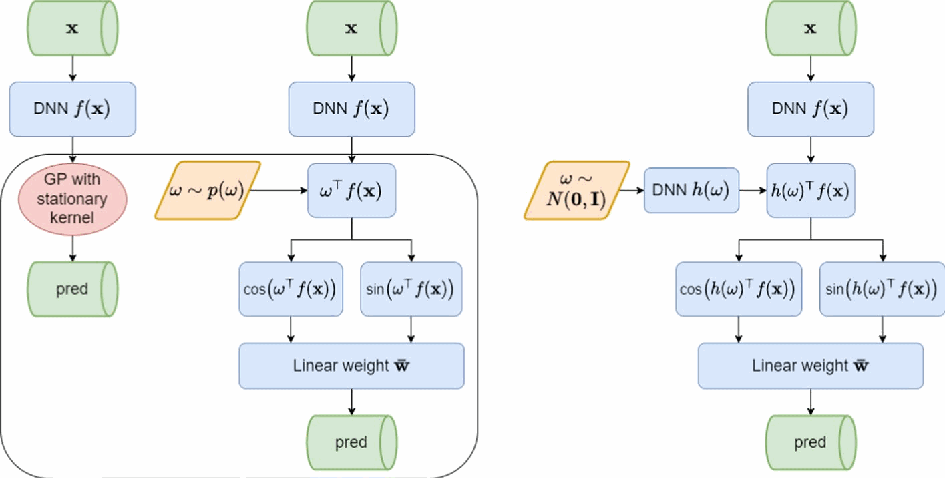
\includegraphics[width=\columnwidth]{fig_2_p10.png}
\caption{From left to right: a standard deep kernel learning algorithm with conventional stationary kernel GPs; the corresponding URK architecture; a more general architecture enabled by URK for convenient latent stationary kernel learning}
\label{fig:2}
\end{figure}
\section{Page 10 of 36}
Machine Learning (2026) 115:72

a fixed number of iterations. Then they send $\theta$ c , $\sigma$ c , and $\lambda$ c back to the server for aggrega tion and start another aggregation round. The local loss function is the negative local log marginal likelihood:

\section{ML}
c = - log Pr BLR ( y c | $\phi$ $\theta$ c ( X c ); $\sigma$ c , $\lambda$ c )

= n c log $\sigma$ 2

c + log( | $\lambda$ 2

\section{c $\bar{}$ w c . (16)}
One commonly used method for aggregation is the FedAvg (McMahan et al., 2017 ) heu ristic, where the new global model parameters are assigned the average of all client model parameters $\theta$ = $\sum$

c $\in$ S $\theta$ c / | S | . However, multiple works (Karimireddy et al., 2020 ; Shoham et al., 2019 ; Mohri et al., 2019 ) have pointed out the quality and the convergence rate of this heuristic can suffer from non-i.i.d. clients. To account for this, we propose to adapt kernel knowledge distillation (He \& Ozay, 2022 ) to aggregate the KNNs. We assume the server holds a relatively small dataset X kd , y kd and tries to minimize the following knowledge distillation loss with respect to this dataset:

\section{KD = L ML kd + $\alpha$ $*$ MSE ( $\phi$ $\theta$ ( X kd ) $^\top$ $\phi$ $\theta$ ( X kd ) ,}
$\sum$

c $\in$ S

$\phi$ $\theta$ c ( X kd ) $^\top$ $\phi$ $\theta$ c ( X kd ) / | S | ) . (17)

here, L ML kd is the log marginal likelihood loss L ML with respect to the knowledge distilla tion dataset X kd , y kd . $\alpha$ is a common hyperparameter in knowledge distillation methods to adjust the ratio between the log marginal likelihood loss and the mean squared error (MSE) loss. The MSE loss forces the global kernel $\phi$ $\theta$ ( X kd ) $^\top$ $\phi$ $\theta$ ( X kd ) to simulate the mean of all client kernels, namely $\sum$

c $\in$ S $\phi$ $\theta$ c ( X kd ) $^\top$ $\phi$ $\theta$ c ( X kd ) / | S | , which is akin to concatenating all the features of the client kernels. Ideally, if the global kernel successfully learns to do so, it should not perform worse on any of the clients, while the FedAvg heuristic has no similar guarantees.

In phase 2, we fix the kernel hyperparameters and learn $\bar{}$ w in an exact way as if all client data is centralized. First, note that we can decompose $\bar{}$ w as follows:

\section{$\bar{}$ w = $\sigma$ - 2 ( $\sigma$ - 2 $\Phi$$\Phi$ $^\top$ + $\lambda$ - 2 I ) - 1 $\Phi$ y (18)}
= $\sigma$ - 2 ( $\sigma$ - 2 $\sum$

\section{c $\in$ S ( $\Phi$ c y c ) (19)}
$\Phi$ c = $\phi$ $\theta$ ( X c ) denotes the random features of local inputs extracted by the global KNN. The server first broadcasts the global model to all the clients and asks them to return the scatter matrices $\Phi$ c $\Phi$ $^\top$ c and the vectors $\Phi$ c y c . Then, the server simply takes the summation of cli ent messages, calculates $\bar{}$ w according to Eq. 19 , and broadcasts the whole model again to all the clients. Note that phase 2 only needs to be done once after kernel learning to achieve the global model. There is no need to iterate between the two phases.

In phase 1, each local update costs O ( n c ( md ) 2 + ( md ) 3 ) time to compute and inverse A c and O (( md ) 2 ) space to store A c . This is equivalent to the complexity of BLR models with random feature approximations. It is more scalable than working with the kernel K directly, which costs O ( n 3 c ) time and O ( n 2 c ) space when md $\ll$ n c . Each client shares a message of size | $\theta$ | with the server. FedAvg aggregation then costs O ( | $\theta$ | ) time and O ( | $\theta$ | ) space, while

Page 11 of 36 72

Machine Learning (2026) 115:72

KD aggregation costs O ( n kd ( md ) 2 + ( md ) 3 + n 2 kd md ) time and O (( md ) 2 + n 2 kd ) space, where n kd is the size of the knowledge distillation dataset. In phase 2, each client calculates the scatter matrices and the vectors, costing O ( n c ( md ) 2 ) time and O (( md ) 2 ) space. Each client shares a message of size ( md ) 2 with the server. Finally, learning the global posterior costs O (( md ) 3 ) time and O (( md ) 2 ) space, similarly to phase 1. Note that if n id inducing points are used to approximate the full kernel (e.g. in pFedGP), O ( n 3 id ) time and O ( n 2 id ) space is needed similarly.

Algorithm 1 Federated Bayesian neural regression ( $\theta$ : the global KNN, $\sigma$ : noise level, $\lambda$ : prior covariance of the linear layer, $\omega$ : a set of random numbers, $\zeta$ : local learning step, $\zeta$ $'$ : knowledge distillation step)

\section{Enhance Protection with DP}
We claim that FedBNR protects the privacy of clients at least as well as FedAvg and other FL algorithms that send client models to the server. In phase 1, the aggregation only requires client model parameters. In phase 2, we send two messages outside each client: $\Phi$ c $\Phi$ $^\top$ c and $\Phi$ c y c . These matrices and vectors (of size m $\times$ m and m ) are also highly compressed summaries of the raw data, which prevents immediate privacy invasions as discussed in Appendix A. We note however that FL with compressed messages does not prevent privacy attacks (Boenisch et al., 2021 ; Mothukuri et al., 2021 ), it simply makes it harder to infer the underlying data. To provide formal privacy guarantees, federated learning needs to be com bined with formal mechanisms such as differential privacy (DP) (Wei et al., 2020 ; Triastcyn \& Faltings, 2019 ) or secure multi-party computation (MPC) (Truex et al., 2019 ; Byrd \& Polychroniadou, 2020 ; Li et al., 2020 ).

\section{Page 12 of 36}
Machine Learning (2026) 115:72

Definition 1 A mechanism M satisfies ( $\epsilon$ , $\delta$ ) -DP if for any two datasets D, D $'$ that differ by only one record (i.e. | ( D - D $'$ ) $\cup$ ( D $'$ - D ) | = 1 , noted as D $\sim$ D $'$ ), and for any possible output O $\in$ Range ( M ) ,

Pr O $\sim$ M ( D )

[

log

( Pr[ M ( D ) = O ]

Pr[ M ( D $'$ ) = O ]

)

> $\epsilon$

] < $\delta$.

The idea of ( $\epsilon$, $\delta$ )-DP is to add enough noise to the shared information so that with high probability ( 0 $\leq$ $\delta$ < 1 ), the distribution of the shared message does not change much when the raw dataset is modified by one record (controlled by $\epsilon$ > 0 ). Thus, one cannot effectively tell if any record is included in the dataset. ( $\epsilon$, $\delta$ )-DP models the information leakage of the raw dataset with the inner log ratio of Def. 1 , and guarantees that it is bounded by $\epsilon$ , the pri vacy budget, with probability $\delta$ . Empirically, people set $\epsilon$ $\leq$ 1 for strong privacy protection, while $\epsilon$ $\geq$ 10 is deemed weak. We will use the following mechanism:

Theorem 3.6 (e.g. (Kerkouche et al., 2021 )). A Gaussian Mechanism GM is ( $\epsilon$, $\delta$ ) -DP with information revealed f: GM ( D ) = f ( D ) + N ( 0 , $\sigma$ 2 I ) , where $\sigma$ = L 2 ( f ) $\sqrt{}$

2 ln( 1 . 25 /$\delta$ ) /$\epsilon$ .

L 2 ( f ) calculates the L 2 sensitivity of function f as follows.

L 2 ( f ) = max

D,D $'$ || f ( D ) - f ( D $'$ ) || 2 , D $\sim$ D $'$ . (20)

We now extend FedBNR to be differentially private with the Gaussian mecha nism. In phase 1, the L 2 sensitivity of the kernel hyperparameters is the L 2 gradi ent clipping constant times the number of local update rounds times the learning rate $\zeta$ . In phase 2, we send [ $\Phi$ c $\Phi$ $^\top$ c , $\Phi$ c y c , y $^\top$ c y c ] instead and its L 2 sensitivity is $\sqrt{}$

32 + 16 /m + 8 b 2 + b 4 , where b := max ( y ) - min ( y ) , assuming the URK construction is g ( $\omega$ , x ) = [sin( $\omega$ $^\top$ $\phi$ NN ( x )) , cos( $\omega$ $^\top$ $\phi$ NN ( x ))] $^\top$ . See details in Appendix A. Then, notice the following matrix is PSD without DP:

\section{[ $\Phi$ c y $^\top$ c}
] [

\section{$\Phi$ $^\top$ c y c}
]

=

\section{[ $\Phi$ c $\Phi$ $^\top$ c $\Phi$ c y c ( $\Phi$ c y c ) $^\top$ y $^\top$}
c y c

] . (21)

After adding Gaussian noise, we project the matrix back to the nearest PSD matrix by set ting its negative eigenvalues to 0. Then we perform regular BLR with projected $\Phi$ c $\Phi$ $^\top$ c and $\Phi$ c y c .

\section{Synthetic Experiments}
We designed the following synthetic experiments to show local GP models cannot handle generalization or new clients . We first decide a true underlying function, sample 200 points uniformly from the range [ - 5 , 5] , and add Gaussian noise with $\sigma$ = 0 . 5 . We then learn the kernel hyperparameters in a centralized fashion to eliminate any impact from imperfect ker

Page 13 of 36 72

Machine Learning (2026) 115:72

nels later on. We assign the first 100 points in range [ - 5 , 0] to client 1, and the rest to client 2. We train pFedGP and FedBNR with the learned kernel hyperparameters fixed and query for prediction in range [ - 5 , 5] . The top left graph of Fig. 3 shows the result of pFedGP, and the top right one shows the result of FedBNR. The blue curve shows the true underlying function, and the green curve shows the predictions. The light red area is a 95\% confidence interval based on variance. The purple dots are the data leveraged by each model for the last layer. Since both algorithms learn hyperparameters centrally, the only difference lies in whether they leverage data of both clients for the predictive model. As shown in the pFedGP graph, the personalized model of client 1 only sees its own data, so it does not generalize well to the range of client 2, while the global model learned by FedBNR leverages all the data and generalizes to the full range.

Next, we introduce two new clients into the system. The first client holds data uniformly sampled from the range [ - 5 , 5] , and the second from the range [5, 15]. We again fix the kernel hyperparameters learned centrally and train pFedGP, FedLoc, and FedBNR on these new clients separately. For testing, we still query the range [ - 5 , 5] . As shown in the bot tom graphs of Fig. 3 . The quality of prediction of the pFedGP model is massively impacted when there are few points in the first case, and for FedBNR the loss remains approximately a straight line. For FedLoc, the loss is also impacted due to zero-out effects of non-over lapping client models. Even worse, when training data and testing data are not in the same range for the second new client, the MSE loss of both pFedGP and FedLoc never drops back to the level of previous clients.

Fig. 3 Top graphs: (i) left: prediction of pFedGP trained on two non-overlapping clients; (ii) right: global prediction of FedBNR. Blue curve: underlying truth; green curve: point estimation; red range: 95\% con fidence interval; purple dots: training data leveraged by the model. Bottom graphs: MSE of predictions tested on the same range v.s. number of training data from a new client; (i) left: client with training range [-5, 5]; (ii) right: client with training range [5, 15]

\section{Page 14 of 36}
Machine Learning (2026) 115:72

\begin{figure}[htbp]
\centering
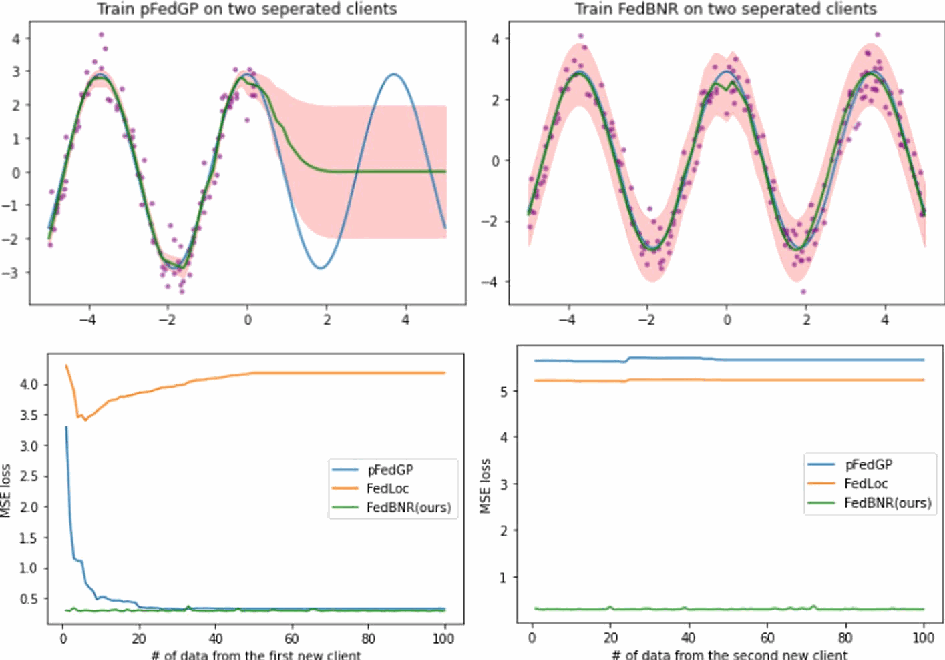
\includegraphics[width=\columnwidth]{fig_3_p14.png}
\caption{Top graphs: (i) left: prediction of pFedGP trained on two non-overlapping clients; (ii) right: global prediction of FedBNR. Blue curve: underlying truth; green curve: point estimation; red range: 95\% con fidence interval; purple dots: training data leveraged by the model. Bottom graphs: MSE of predictions tested on the same range v.s. number of training data from a new client; (i) left: client with training range [-5, 5]; (ii) right: client with training range [5, 15]}
\label{fig:3}
\end{figure}
\section{Real World Regression Tasks}
To show our algorithm achieves better generalization performance in terms of both point and uncertainty estimation , we conducted comprehensive experiments on 5 real world regression tasks under 10 cases, including Skillcraft (Thompson et al., 2013 ), SML (Zamora-Martinez et al., 2014 ), Parkinsons (Tsanas et al., 2009 ), Bike (VE \& Cho, 2020 ), and CCPP (Tüfekci, 2014 ). We note while a common challenge for GPs is to scale to large datasets, in FL, the challenge is the opposite: how to combine models trained on small datasets. When the datasets of each client become sufficiently large, then there is no need to combine models nor do FL. Hence, the experiments focus on reducing the amount of data per client while increasing the number of clients. The scalability of FedBNR is trivially guaranteed by the use of random features. Results of two variants are reported: (i) FedBNR that performs the FedAvg heuristic at aggregation; and (ii) FedBNR-KD that performs the knowledge distillation method at aggregation. Two groups of baselines are compared to our method for RMSE error: (i) ablation study that includes local+local, local+global, avg+local, and kd+global, in the format of kernel learning method + last linear weight learning method, where we remove the global aggregation of either Phase 1 or Phase 2 from our methods; (ii) previous works that include (1) FedAvg (McMahan et al., 2017 ), a standard non-Bayesian FL algorithm that has a global model; (2) FedProx (Li et al., 2020 ), a non-Bayesian FL algorithm that adds a proximal loss to FedAvg to prevent client models from getting too far from the global model; (3) pFedGP (Achituve et al., 2021 ), a Bayesian PFL method that learns a local GP with a shared deep kernel for each client using FedAvg; (4) FedLoc (Yin et al., 2020 ), a Bayesian FL method that directly applies distributed GP methods (Xie et al., 2019 ) without deep kernel learning; (5) DEC-apx-GP (Kontoudis \& Stilwell, 2023 ), a decentralized Bayesian PFL method that learns a local GP with a shared separable squared exponential kernel for each client using proximal ADMM; and (6) DEC-gapx-GP (Kon toudis \& Stilwell, 2024 ), an extension of DEC-apx-GP that shares an additional dataset with all clients as extra training data. We also compare to pFedGP, FedLoc, DEC-apx, and DEC- gapx for calibration errors since they are Bayesian models that have a notion of confidence. Besides, we report results of a centralized GP equipped with URK as a casual reference of the testing error lower bound. We used fully connected neural networks to extract first- step features for FedAvg, FedProx, and pFedGP. We used Gaussian kernels for the GPs in pFedGP and FedLoc. For fairness, KNNs used by our methods have similar architectures to the combined kernel of pFedGP. FITC (Snelson \& Ghahramani, 2005 ) approximations are implemented for pFedGP and FedLoc as described in pFedGP. We used 50 random samples for KNN and 50 inducing points for pFedGP and FedLoc. Further details are in Appendix B.

Each dataset is uniformly divided into training, testing, and validation sets globally with a ratio of 8:1:1. The training data is sorted by the feature that has the largest absolute cor relation coefficient with the output, and divided into multiple chunks. Each client randomly takes two chunks so their data distributions are heterogeneous. The larger the absolute cor relation coefficient is, the more significant the distribution skew is. Before training, we tune hyperparameters that cannot be learned by gradient descent with grid searching on the validation set. Specially, FedBNR-KD uses 80\% of the validation set for knowledge distil lation, and the rest 20\% for validation. All datasets are ran for 50 local epochs times at most 100 aggregation rounds in full batches. Validation and testing errors are recorded for each aggregation round. For methods that contain only local models, these errors are defined as

Page 15 of 36 72

Machine Learning (2026) 115:72

the mean error of all local models with respect to the testing/validation set. If the validation error has not improved for 5 rounds, the training process is terminated.

We report the average minimum testing RMSE for 10 random seeds for each case in Table 1 , which assesses the point estimation of different models. We also measured the statistical significance of the results compared to FedBNR with one-tailed Wilcoxon signed- rank tests (Wilcoxon, 1992 ). We report expected calibration errors (ECE) in Table 2 and per form the Wilcoxon test compared to FedBNR-KD. ECE is a calibration metric that assesses the uncertainty estimation. Further metrics are included in Appendix C.

The results show: (i) in terms of RMSE, our methods are statistically better than the other models in most of the cases, especially when the training set at each client is significantly smaller than the whole set; (ii) compared with the ablation study methods, our methods always perform better, so the global aggregation at both phases is essential; (iii) FedLoc without deep kernel has a much smaller model capacity; (iv) FedBNR-KD only outperforms FedBNR in 40\% of cases in terms of RMSE, which is probably due to the small size of data (8\% of all) used for knowledge distillation. However, it is clearly more stable when client heterogeneity gets worse as the number of clients increases. It is also better calibrated in most cases.

\begin{table}[htbp]
\centering
\small
\caption{ECE reported for the generalization setting. $\Uparrow$ , $\uparrow$ , $\Downarrow$ , and $\downarrow$ denote significantly worse or better results similarly to Table 1}
\resizebox{\columnwidth}{!}{%
\begin{tabular}{|l|l|l|l|l|l|l|l|l|l|l|l|l|l|l|l|l|l|l|l|l|l|l|l|l|l|l|l|l|l|l|l|l|l|l|l|l|l|l|l|l|}
\hline
\textbf{Skillcraft} & \textbf{SML} & \textbf{Parkinsons} & \textbf{Bike} & \textbf{CCPP} & \textbf{\#Clients} & \textbf{10} & \textbf{100} & \textbf{10} & \textbf{100} & \textbf{10} & \textbf{100} & \textbf{10} & \textbf{100} & \textbf{10} & \textbf{100} & \textbf{Central} & \textbf{GP} & \textbf{0.02} & \textbf{0.09} & \textbf{0.27} & \textbf{0.11} & \textbf{0.24} \\
\hline
pFedGP & 0 & . & 43 & $\Uparrow$ & 0 & . & 38 & $\Uparrow$ & 0 & . & 45 & $\Uparrow$ & 0 & . & 45 & $\Uparrow$ & 0 & . & 49 & $\Uparrow$ & 0 & . & 48 & $\Uparrow$ & 0 & . & 42 & $\Uparrow$ & 0 & . & 41 & $\Uparrow$ & 0 & . & 49 & $\Uparrow$ & 0 & . & 49 & $\Uparrow$ \\
FedLoc & 0 & . & 32 & $\Uparrow$ & 0 & . & 44 & $\Uparrow$ & 0 & . & 12 & $\Downarrow$ & 0 & . & 27 & $\Uparrow$ & 0 & . & 32 & $\Uparrow$ & 0 & . & 43 & $\Uparrow$ & 0 & . & 26 & $\Uparrow$ & 0 & . & 16 & $\Uparrow$ & 0 & . & 23 & $\Downarrow$ & 0 & . & 50 & $\Uparrow$ \\
DEC-apx & 0 & . & 50 & $\Uparrow$ & 0 & . & 46 & $\Uparrow$ & 0 & . & 50 & $\Uparrow$ & 0 & . & 50 & $\Uparrow$ & 0 & . & 50 & $\Uparrow$ & 0 & . & 50 & $\Uparrow$ & 0 & . & 19 & $\Uparrow$ & 0 & . & 14 & $\Uparrow$ & 0 & . & 42 & $\Uparrow$ & 0 & . & 38 & $\Uparrow$ \\
DEC-gapx & 0 & . & 50 & $\Uparrow$ & 0 & . & 36 & $\Uparrow$ & 0 & . & 50 & $\Uparrow$ & 0 & . & 50 & $\Uparrow$ & 0 & . & 50 & $\Uparrow$ & 0 & . & 50 & $\Uparrow$ & 0 & . & 28 & $\Uparrow$ & 0 & . & 19 & $\Uparrow$ & 0 & . & 47 & $\Uparrow$ & 0 & . & 42 & $\Uparrow$ \\
ours & FedBNR & 0 & . & 05 & 0 & . & 20 & $\Uparrow$ & 0 & . & 39 & $\Uparrow$ & 0 & . & 37 & $\Uparrow$ & 0 & . & 36 & $\uparrow$ & 0 & . & 40 & $\Uparrow$ & 0 & . & 07 & 0 & . & 04 & $\Uparrow$ & 0 & . & 24 & $\Downarrow$ & 0 & . & 20 & $\Downarrow$ &  \\
FedBNR-KD & 0 & . & 05 & 0 & . & 06 & 0.20 & 0 & . & 21 & 0 & . & 29 & 0 & . & 30 & 0.08 & 0 & . & 09 & 0.30 & 0.31 &  &  &  &  &  &  &  &  &  &  &  &  &  &  &  &  &  &  \\
\hline
\end{tabular}
}
\end{table}
\section{Personalization}
We conducted experiments with the personalization setting to show that the global GP posterior benefits uncertainty estimation even in the personalization setting . FedBNR can be naturally extended to the personalization setting by fine-tuning the global model. During fine-tuning, we minimize L F T c = || y c - $\phi$ $\theta$ c ( X c ) w c || 2 2 + $\lambda$ - 2 c || w c || 2 2 , the local regu

Skillcraft SML Parkinsons Bike CCPP Train/test size 2670/334 3309/414 4700/587 7008/876 7654/957 corr-coef - 0.660 0.783 0.410 0.539 - 0.948 \#clients 10 100 10 100 10 100 10 100 10 100 Central GP 0.95 0.21 3.58 0.37 4.02

\section{Page 16 of 36}
Machine Learning (2026) 115:72

larized least square loss. Note the weights in the last linear layer are also updated by gradient descent. Varying the number of epochs of fine-tuning offers a controllable trade-off between generalization and personalization. Training datasets are distributed to clients as before for heterogeneity, but testing and validation sets are sampled with the same distribution as local training datasets, with a ratio of 14:3:3. We report the RMSE and ECE in Table 3 , where pxADMM (Xie et al., 2019 ) is a distributed GP hyperparameter learning algorithm used by FedLoc and we extend it with deep kernels. The results show that FedBNR achieves compa rable accuracy and better calibration than other methods, indicating a global posterior helps calibrate local models.

\section{Differential Privacy}
We conducted experiments for FedBNR with DP to show the trade-off between model utility and the privacy budget $\epsilon$ . Experiment details are similar to Sect. 4.2 . The results of the Skillcraft and SML datasets are summarized in Fig. 4 . As the graph shows, the RMSE loss of fully differentially private FedBNR quickly drops back to the RMSE of vanilla Fed Log, when $\epsilon$ $\geq$ 0 . 1 . The DP noise affects the model less when there are more clients, since in Phase 1 the messages are averaged. Extra results are in Appendix C.

\begin{table}[htbp]
\centering
\small
\caption{Real world regression datasets, RMSE reported for the generalization setting. $\Uparrow$ and $\uparrow$ denote sig nificantly worse results with p < 0 . 01 and p < 0 . 05 respectively; $\Downarrow$ and $\downarrow$ denote significantly better results similarly}
\resizebox{\columnwidth}{!}{%
\begin{tabular}{|l|l|l|l|l|l|l|l|l|l|l|l|l|l|l|l|l|l|l|l|l|l|l|l|l|l|l|l|l|l|l|l|l|l|l|l|l|l|l|l|l|l|l|l|l|l|l|l|l|l|l|l|l|l|l|l|l|l|l|l|l|l|l|l|l|l|l|l|l|l|l|l|l|l|l|l|l|l|l|l|l|l|l|l|l|l|l|l|l|l|l|l|l|l|l|l|l|l|l|l|l|l|l|l|l|l|l|l|l|l|l|l|l|l|l|l|l|l|l|l|}
\hline
\textbf{Skillcraft} & \textbf{SML} & \textbf{Parkinsons} & \textbf{Bike} & \textbf{CCPP} & \textbf{Train/test} & \textbf{size} & \textbf{2670/334} & \textbf{3309/414} & \textbf{4700/587} & \textbf{7008/876} & \textbf{7654/957} & \textbf{corr-coef} & \textbf{-} & \textbf{0.660} & \textbf{0.783} & \textbf{0.410} & \textbf{0.539} & \textbf{-} & \textbf{0.948} & \textbf{\#clients} & \textbf{10} & \textbf{100} & \textbf{10} & \textbf{100} & \textbf{10} & \textbf{100} & \textbf{10} & \textbf{100} & \textbf{10} & \textbf{100} & \textbf{Central} & \textbf{GP} & \textbf{0.95} & \textbf{0.21} & \textbf{3.58} & \textbf{0.37} & \textbf{4.02} \\
\hline
Local+local & 1 & . & 26 & $\Uparrow$ & 1 & . & 48 & $\Uparrow$ & 1 & . & 49 & $\Uparrow$ & 2 & . & 32 & $\Uparrow$ & 10 & . & 9 & $\Uparrow$ & 10 & . & 6 & $\Uparrow$ & 0 & . & 79 & $\Uparrow$ & 0 & . & 92 & $\Uparrow$ & 14 & . & 6 & $\Uparrow$ & 19 & . & 3 & $\Uparrow$ &  &  &  &  &  &  &  &  &  &  &  &  &  &  &  &  &  &  &  &  &  &  &  &  &  &  &  &  &  &  &  &  &  &  &  &  &  &  &  &  &  &  &  &  &  &  &  &  &  &  &  &  &  &  &  &  &  &  &  &  &  &  &  &  &  &  &  &  &  &  &  &  &  &  &  &  &  &  &  \\
Local+global & 1 & . & 08 & $\Uparrow$ & 1 & . & 22 & $\Uparrow$ & 1 & . & 00 & $\Uparrow$ & 1 & . & 65 & $\Uparrow$ & 6 & . & 42 & $\Uparrow$ & 7 & . & 42 & $\Uparrow$ & 0 & . & 59 & $\Uparrow$ & 0 & . & 73 & $\Uparrow$ & 5 & . & 62 & $\Uparrow$ & 7 & . & 03 & $\Uparrow$ &  &  &  &  &  &  &  &  &  &  &  &  &  &  &  &  &  &  &  &  &  &  &  &  &  &  &  &  &  &  &  &  &  &  &  &  &  &  &  &  &  &  &  &  &  &  &  &  &  &  &  &  &  &  &  &  &  &  &  &  &  &  &  &  &  &  &  &  &  &  &  &  &  &  &  &  &  &  &  \\
Avg+local & 1 & . & 05 & $\Uparrow$ & 1 & . & 06 & $\Uparrow$ & 0 & . & 61 & $\Uparrow$ & 0 & . & 81 & $\Uparrow$ & 9 & . & 84 & $\Uparrow$ & 8 & . & 80 & $\Uparrow$ & 0 & . & 45 & $\Uparrow$ & 0 & . & 54 & $\Uparrow$ & 8 & . & 32 & $\Uparrow$ & 13 & . & 4 & $\Uparrow$ &  &  &  &  &  &  &  &  &  &  &  &  &  &  &  &  &  &  &  &  &  &  &  &  &  &  &  &  &  &  &  &  &  &  &  &  &  &  &  &  &  &  &  &  &  &  &  &  &  &  &  &  &  &  &  &  &  &  &  &  &  &  &  &  &  &  &  &  &  &  &  &  &  &  &  &  &  &  &  \\
kd+local & 1 & . & 04 & $\Uparrow$ & 1 & . & 28 & $\Uparrow$ & 0 & . & 86 & $\Uparrow$ & 1 & . & 34 & $\Uparrow$ & 6 & . & 15 & $\Uparrow$ & 6 & . & 97 & $\Uparrow$ & 0 & . & 51 & $\Uparrow$ & 0 & . & 61 & $\Uparrow$ & 10 & . & 0 & $\Uparrow$ & 17 & . & 1 & $\Uparrow$ &  &  &  &  &  &  &  &  &  &  &  &  &  &  &  &  &  &  &  &  &  &  &  &  &  &  &  &  &  &  &  &  &  &  &  &  &  &  &  &  &  &  &  &  &  &  &  &  &  &  &  &  &  &  &  &  &  &  &  &  &  &  &  &  &  &  &  &  &  &  &  &  &  &  &  &  &  &  &  \\
FedAvg & 1 & . & 00 & $\uparrow$ & 1 & . & 03 & $\Uparrow$ & 0 & . & 36 & $\Uparrow$ & 0 & . & 71 & $\Uparrow$ & 6 & . & 83 & $\Uparrow$ & 7 & . & 38 & $\Uparrow$ & 0 & . & 38 & $\downarrow$ & 0.42 & 4.45 & 4.44 &  &  &  &  &  &  &  &  &  &  &  &  &  &  &  &  &  &  &  &  &  &  &  &  &  &  &  &  &  &  &  &  &  &  &  &  &  &  &  &  &  &  &  &  &  &  &  &  &  &  &  &  &  &  &  &  &  &  &  &  &  &  &  &  &  &  &  &  &  &  &  &  &  &  &  &  &  &  &  &  &  &  &  &  &  &  &  &  \\
FedProx & 0.98 & 1 & . & 05 & $\Uparrow$ & 0 & . & 34 & $\uparrow$ & 0 & . & 62 & $\Uparrow$ & 6 & . & 32 & $\Uparrow$ & 7 & . & 38 & $\Uparrow$ & 0.39 & 0.42 & 4.43 & 4.47 &  &  &  &  &  &  &  &  &  &  &  &  &  &  &  &  &  &  &  &  &  &  &  &  &  &  &  &  &  &  &  &  &  &  &  &  &  &  &  &  &  &  &  &  &  &  &  &  &  &  &  &  &  &  &  &  &  &  &  &  &  &  &  &  &  &  &  &  &  &  &  &  &  &  &  &  &  &  &  &  &  &  &  &  &  &  &  &  &  &  &  &  &  &  \\
pFedGP & 0 & . & 99 & $\uparrow$ & 1 & . & 15 & $\Uparrow$ & 0 & . & 75 & $\Uparrow$ & 1 & . & 34 & $\Uparrow$ & 9 & . & 36 & $\Uparrow$ & 8 & . & 91 & $\Uparrow$ & 0 & . & 45 & $\Uparrow$ & 0 & . & 46 & $\Uparrow$ & 14 & . & 2 & $\Uparrow$ & 18 & . & 2 & $\Uparrow$ &  &  &  &  &  &  &  &  &  &  &  &  &  &  &  &  &  &  &  &  &  &  &  &  &  &  &  &  &  &  &  &  &  &  &  &  &  &  &  &  &  &  &  &  &  &  &  &  &  &  &  &  &  &  &  &  &  &  &  &  &  &  &  &  &  &  &  &  &  &  &  &  &  &  &  &  &  &  &  \\
FedLoc & 1 & . & 08 & $\Uparrow$ & 4 & . & 15 & $\Uparrow$ & 2 & . & 83 & $\Uparrow$ & 5 & . & 43 & $\Uparrow$ & 8 & . & 40 & $\Uparrow$ & 11 & . & 5 & $\Uparrow$ & 0 & . & 64 & $\Uparrow$ & 0 & . & 75 & $\Uparrow$ & 20 & . & 6 & $\Uparrow$ & 44 & . & 1 & $\Uparrow$ &  &  &  &  &  &  &  &  &  &  &  &  &  &  &  &  &  &  &  &  &  &  &  &  &  &  &  &  &  &  &  &  &  &  &  &  &  &  &  &  &  &  &  &  &  &  &  &  &  &  &  &  &  &  &  &  &  &  &  &  &  &  &  &  &  &  &  &  &  &  &  &  &  &  &  &  &  &  &  \\
DEC-apx & 1 & . & 10 & $\Uparrow$ & 4 & . & 34 & $\Uparrow$ & 1 & . & 90 & $\Uparrow$ & 4 & . & 93 & $\Uparrow$ & 8 & . & 59 & $\Uparrow$ & 9 & . & 21 & $\Uparrow$ & 0 & . & 76 & $\Uparrow$ & 0 & . & 88 & $\Uparrow$ & 7 & . & 64 & $\Uparrow$ & 11 & . & 06 & $\Uparrow$ &  &  &  &  &  &  &  &  &  &  &  &  &  &  &  &  &  &  &  &  &  &  &  &  &  &  &  &  &  &  &  &  &  &  &  &  &  &  &  &  &  &  &  &  &  &  &  &  &  &  &  &  &  &  &  &  &  &  &  &  &  &  &  &  &  &  &  &  &  &  &  &  &  &  &  &  &  &  &  \\
DEC-gapx & 0 & . & 94 & $\Downarrow$ & 4 & . & 31 & $\Uparrow$ & 1 & . & 41 & $\Uparrow$ & 3 & . & 57 & $\Uparrow$ & 8 & . & 07 & $\Uparrow$ & 8 & . & 26 & $\Uparrow$ & 0 & . & 55 & $\Uparrow$ & 0 & . & 75 & $\Uparrow$ & 6 & . & 26 & $\Uparrow$ & 9 & . & 12 & $\Uparrow$ &  &  &  &  &  &  &  &  &  &  &  &  &  &  &  &  &  &  &  &  &  &  &  &  &  &  &  &  &  &  &  &  &  &  &  &  &  &  &  &  &  &  &  &  &  &  &  &  &  &  &  &  &  &  &  &  &  &  &  &  &  &  &  &  &  &  &  &  &  &  &  &  &  &  &  &  &  &  &  \\
ours & FedBNR & 0.98 & 0 & . & 97 & 0 & . & 25 & 0 & . & 44 & 3 & . & 10 & 5.42 & 0.39 & 0 & . & 42 & 4.40 & 4.51 & FedBNR-KD & 0 & . & 96 & $\Downarrow$ & 0 & . & 98 & $\uparrow$ & 0 & . & 55 & $\Uparrow$ & 0 & . & 55 & $\Uparrow$ & 4 & . & 58 & $\Uparrow$ & 4 & . & 67 & $\downarrow$ & 0 & . & 43 & $\Uparrow$ & 0 & . & 48 & $\Uparrow$ & 4 & . & 38 & 4 & . & 38 & $\downarrow$ &  &  &  &  &  &  &  &  &  &  &  &  &  &  &  &  &  &  &  &  &  &  &  &  &  &  &  &  &  &  &  &  &  &  &  &  &  &  &  &  &  &  &  &  &  &  &  &  &  &  &  &  &  &  &  &  &  &  \\
larized & least & square & loss. & Note & the & weights & in & the & last & linear & layer & are & also & updated & by & gradient & descent. & Varying & the & number & of & epochs & of & fine-tuning & offers & a & controllable & trade-off & between & generalization & and & personalization. & Training & datasets & are & distributed & to & clients & as & before & for & heterogeneity, & but & testing & and & validation & sets & are & sampled & with & the & same & distribution & as & local & training & datasets, & with & a & ratio & of & 14:3:3. & We & report & the & RMSE & and & ECE & in & Table & 3 & , & where & pxADMM & (Xie & et & al., & 2019 & ) & is & a & distributed & GP & hyperparameter & learning & algorithm & used & by & FedLoc & and & we & extend & it & with & deep & kernels. & The & results & show & that & FedBNR & achieves & compa & rable & accuracy & and & better & calibration & than & other & methods, & indicating & a & global & posterior & helps & calibrate & local & models. \\
\hline
\end{tabular}
}
\end{table}
\begin{table}[htbp]
\centering
\small
\caption{RMSE (top half) and ECE (bottom half) reported for the personalization setting. $\Uparrow$ and $\uparrow$ denote significantly worse results with p < 0 . 01 and p < 0 . 05 respectively; $\Downarrow$ and $\downarrow$ denote significantly better results similarly \#Clients Skillcraft SML Parkinsons Bike CCPP 10 100 10 100 10 100 10 100 10 100 pFedGP 1 . 00 $\Downarrow$ 1 . 08 $\Downarrow$ 0 . 31 $\Uparrow$ 0.64 2 . 97 $\Uparrow$ 3 . 66 $\Uparrow$ 0 . 47 0 . 44 $\Downarrow$ 4 . 72 $\Uparrow$ 12 . 66 $\Uparrow$}
\resizebox{\columnwidth}{!}{%
\begin{tabular}{|l|l|l|l|l|l|l|l|l|l|l|l|l|l|l|l|l|l|l|l|l|l|l|l|l|l|l|l|l|l|l|l|l|l|l|l|l|l|l|l|l|l|l|l|l|l|l|l|l|l|l|l|l|l|l|l|l|l|}
\hline
\textbf{pxADMM} & \textbf{0} & \textbf{.} & \textbf{99} & \textbf{$\Downarrow$} & \textbf{1} & \textbf{.} & \textbf{16} & \textbf{$\Downarrow$} & \textbf{2} & \textbf{.} & \textbf{11} & \textbf{$\Uparrow$} & \textbf{1} & \textbf{.} & \textbf{75} & \textbf{$\Uparrow$} & \textbf{6} & \textbf{.} & \textbf{99} & \textbf{$\Uparrow$} & \textbf{3} & \textbf{.} & \textbf{73} & \textbf{$\Uparrow$} & \textbf{0} & \textbf{.} & \textbf{56} & \textbf{$\Uparrow$} & \textbf{0} & \textbf{.} & \textbf{50} & \textbf{$\Downarrow$} & \textbf{10} & \textbf{.} & \textbf{21} & \textbf{$\Uparrow$} & \textbf{14} & \textbf{.} & \textbf{60} & \textbf{$\Uparrow$} \\
\hline
DEC-apx & 1.10 & 4 & . & 19 & $\Uparrow$ & 1 & . & 59 & $\Uparrow$ & 3 & . & 49 & $\Uparrow$ & 3 & . & 56 & $\Uparrow$ & 3 & . & 32 & $\Uparrow$ & 0 & . & 57 & $\Uparrow$ & 0 & . & 71 & $\Uparrow$ & 4 & . & 40 & $\Uparrow$ & 4 & . & 92 & $\Uparrow$ &  &  &  &  &  &  &  &  &  &  &  &  &  &  &  &  &  &  &  &  \\
DEC-gapx & 0 & . & 96 & $\Downarrow$ & 2 & . & 91 & $\Uparrow$ & 1 & . & 15 & $\Uparrow$ & 3 & . & 30 & $\Uparrow$ & 4 & . & 49 & $\Uparrow$ & 5 & . & 83 & $\Uparrow$ & 0 & . & 54 & $\Uparrow$ & 0 & . & 64 & $\Uparrow$ & 4 & . & 40 & $\Uparrow$ & 5 & . & 74 & $\Uparrow$ &  &  &  &  &  &  &  &  &  &  &  &  &  &  &  &  &  \\
ours & FedBNR & 1.12 & 1.25 & 0 & . & 25 & 0 & . & 62 & 1 & . & 39 & 1 & . & 75 & 0 & . & 47 & 0.57 & 3 & . & 89 & 4.77 & FedBNR-KD & 1.12 & 1 & . & 22 & $\Downarrow$ & 0 & . & 38 & $\Uparrow$ & 0.66 & 1 & . & 78 & $\Uparrow$ & 2 & . & 13 & $\Uparrow$ & 0 & . & 49 & $\Uparrow$ & 0 & . & 63 & $\Uparrow$ & 3 & . & 95 & $\Uparrow$ & 4 & . & 74 \\
\#Clients & Skillcraft & SML & Parkinsons & Bike & CCPP & 10 & 100 & 10 & 100 & 10 & 100 & 10 & 100 & 10 & 100 & pFedGP & 0 & . & 42 & $\Uparrow$ & 0 & . & 35 & $\Uparrow$ & 0 & . & 45 & $\Uparrow$ & 0 & . & 44 & $\Uparrow$ & 0 & . & 45 & $\Uparrow$ & 0 & . & 44 & $\Uparrow$ & 0 & . & 42 & $\Uparrow$ & 0 & . & 39 & $\Uparrow$ & 0 & . & 49 & $\Uparrow$ & 0 & . & 49 & $\Uparrow$ &  \\
pxADMM & 0 & . & 42 & $\Uparrow$ & 0 & . & 34 & $\Uparrow$ & 0 & . & 50 & $\Uparrow$ & 0 & . & 45 & $\Uparrow$ & 0 & . & 49 & $\Uparrow$ & 0 & . & 44 & $\Uparrow$ & 0 & . & 20 & $\Uparrow$ & 0 & . & 21 & $\Uparrow$ & 0 & . & 50 & $\Uparrow$ & 0 & . & 49 & $\Uparrow$ &  &  &  &  &  &  &  &  &  &  &  &  &  &  &  &  &  \\
DEC-apx & 0 & . & 50 & $\Uparrow$ & 0 & . & 50 & $\Uparrow$ & 0 & . & 50 & $\Uparrow$ & 0 & . & 50 & $\Uparrow$ & 0 & . & 50 & $\Uparrow$ & 0 & . & 50 & $\Uparrow$ & 0 & . & 27 & $\Uparrow$ & 0 & . & 21 & $\Uparrow$ & 0 & . & 27 & $\Uparrow$ & 0 & . & 43 & $\Uparrow$ &  &  &  &  &  &  &  &  &  &  &  &  &  &  &  &  &  \\
DEC-gapx & 0 & . & 50 & $\Uparrow$ & 0 & . & 50 & $\Uparrow$ & 0 & . & 50 & $\Uparrow$ & 0 & . & 50 & $\Uparrow$ & 0 & . & 45 & $\Uparrow$ & 0 & . & 50 & $\Uparrow$ & 0 & . & 28 & $\Uparrow$ & 0 & . & 24 & $\Uparrow$ & 0 & . & 20 & $\Downarrow$ & 0 & . & 12 & $\Downarrow$ &  &  &  &  &  &  &  &  &  &  &  &  &  &  &  &  &  \\
ours & FedBNR & 0 & . & 01 & 0.04 & 0.24 & 0.28 & 0 & . & 04 & 0 & . & 04 & 0 & . & 11 & 0.08 & 0.25 & 0.33 & FedBNR-KD & 0 & . & 01 & 0 & . & 03 & $\Downarrow$ & 0 & . & 13 & $\Downarrow$ & 0 & . & 17 & $\Downarrow$ & 0 & . & 06 & $\Uparrow$ & 0 & . & 09 & $\Uparrow$ & 0 & . & 11 & 0 & . & 07 & 0 & . & 29 & $\Uparrow$ & 0.33 &  &  &  \\
Fig. & 4 & FedBNR+DP & results. & Left: & Skillcraft & dataset; & right: & SML & dataset. & Phase & 1 & DP: & add & DP & protection & to & $\theta$ & c & only; & full & DP: & add & DP & protection & to & all & messages &  &  &  &  &  &  &  &  &  &  &  &  &  &  &  &  &  &  &  &  &  &  &  &  &  &  &  &  &  &  \\
with & them. & We & then & discuss & privacy & leakage & of & different & GP & algorithms & and & summarize & them & in & Table & 4 & . & We & will & now & discuss & messages & and & algorithms & listed & in & the & table & one & by & one. &  &  &  &  &  &  &  &  &  &  &  &  &  &  &  &  &  &  &  &  &  &  &  &  &  &  \\
\hline
\end{tabular}
}
\end{table}
\begin{table}[htbp]
\centering
\small
\caption{Privacy leakage of dif ferent GP algorithms Risky message: messages that leak privacy but unavoidable for global prediction. Problematic term: terms that the risky messages try to compute. Leaked info: private information that can be recovered by adversaries with the risky messages. $\subset$ means ``part of''}
\resizebox{\columnwidth}{!}{%
\begin{tabular}{|l|l|l|l|l|l|l|l|l|l|l|l|l|l|l|l|l|l|l|l|l|l|l|l|l|l|l|l|l|l|l|l|}
\hline
\textbf{Then} & \textbf{the} & \textbf{adversaries} & \textbf{can} & \textbf{again} & \textbf{retrieve} & \textbf{y} & \textbf{c} & \textbf{=} & \textbf{k} & \textbf{(} & \textbf{X} & \textbf{c} & \textbf{,} & \textbf{U} & \textbf{)} & \textbf{$\Sigma$} & \textbf{k} & \textbf{(} & \textbf{U} & \textbf{,} & \textbf{X} & \textbf{)} & \textbf{$\Lambda$} & \textbf{-} & \textbf{1} & \textbf{y} & \textbf{without} & \textbf{knowing} & \textbf{X} & \textbf{c} & \textbf{.} \\
\hline
FedAvg & FedAvg & shares & no & risky & messages & listed & before. & It & shares & model & parameters & only. &  &  &  &  &  &  &  &  &  &  &  &  &  &  &  &  &  &  &  \\
\hline
\end{tabular}
}
\end{table}
\begin{table}[htbp]
\centering
\small
\caption{Hyperparameters used in the real world regression experiments. For FedLoc L = 10 $\rho$ to run the Proximal ADMM algorithm \#Clients Skillcraft SML Parkinsons Bike CCPP 10 100 10 100 10 100 10 100 10 100 Size s 200 2000 2000 5000 5000 FedProx $\mu$ 0.5 1.0 0.1 1.0 1.0 1.0 0.1 0.01 0.001 1.0 FedLoc $\rho$ 5e3 5e4 5e3 5e4 1e3 5e3 5e4 5e4 1e5 1e5 FedBNR-KD $\alpha$ 10 2 1 0.5 5 2 5 0.5 5 5}
\resizebox{\columnwidth}{!}{%
\begin{tabular}{|l|l|l|l|l|l|l|l|l|l|l|l|l|l|l|l|l|l|l|l|l|l|l|l|l|l|l|l|l|l|l|l|l|l|l|l|l|l|l|l|l|l|l|l|l|l|l|l|l|l|l|l|l|l|l|l|l|l|l|l|l|l|l|l|}
\hline
\textbf{URK} & \textbf{m} & \textbf{$\omega$,g} & \textbf{(} & \textbf{x} & \textbf{,} & \textbf{x} & \textbf{$'$} & \textbf{)} & \textbf{=} \\
\hline
s & m & $\omega$ & ( & x & ) & $\sqrt{}$ & m &  &  &  &  &  &  &  &  &  &  &  &  &  &  &  &  &  &  &  &  &  &  &  &  &  &  &  &  &  &  &  &  &  &  &  &  &  &  &  &  &  &  &  &  &  &  &  &  &  &  &  &  &  &  &  &  \\
) & $^\top$ & ( &  &  &  &  &  &  &  &  &  &  &  &  &  &  &  &  &  &  &  &  &  &  &  &  &  &  &  &  &  &  &  &  &  &  &  &  &  &  &  &  &  &  &  &  &  &  &  &  &  &  &  &  &  &  &  &  &  &  &  &  &  \\
s & m & $\omega$ & ( & x & $'$ & ) & $\sqrt{}$ & m &  &  &  &  &  &  &  &  &  &  &  &  &  &  &  &  &  &  &  &  &  &  &  &  &  &  &  &  &  &  &  &  &  &  &  &  &  &  &  &  &  &  &  &  &  &  &  &  &  &  &  &  &  &  &  \\
1 & m & ( & g & ( & $\omega$ & i & , & x & ) & $^\top$ & g & ( & $\omega$ & i & , & x & $'$ & )) &  &  &  &  &  &  &  &  &  &  &  &  &  &  &  &  &  &  &  &  &  &  &  &  &  &  &  &  &  &  &  &  &  &  &  &  &  &  &  &  &  &  &  &  &  \\
g & ( & $\omega$ & i & , & x & ) & $^\top$ & g & ( & $\omega$ & i & , & x & $'$ & ) & are & i.i.d. & 1-dimensional & random & variables. & It & is & bounded & by & [ & - & 2 & , & 2] & since & g & ( & $\omega$ & , & x & ) & = & [sin( & $\omega$ & $^\top$ & $\phi$ & NN & ( & x & )) & , & cos( & $\omega$ & $^\top$ & $\phi$ & NN & ( & x & ))] & $^\top$ & . & Finally, & apply & the & Hoeffding's & inequality. &  & $\square$ \\
Approximate & Non-stationary & Kernels & Without & DNN &  &  &  &  &  &  &  &  &  &  &  &  &  &  &  &  &  &  &  &  &  &  &  &  &  &  &  &  &  &  &  &  &  &  &  &  &  &  &  &  &  &  &  &  &  &  &  &  &  &  &  &  &  &  &  &  &  &  &  \\
\hline
\end{tabular}
}
\end{table}
\begin{table}[htbp]
\centering
\small
\caption{RMSE reported. Generalization setting. FedBNR \textbackslash\{\} URK: removing random features from FedBNR; FedBNR: ordinary FedBNR. $\Uparrow$ and $\uparrow$ denote significantly worse results with p < 0 . 01 and p < 0 . 05 respec tively; $\Downarrow$ and $\downarrow$ denote significantly better results similarly \#Clients Skillcraft SML Parkinsons Bike CCPP 10 100 10 100 10 100 10 100 10 100}
\resizebox{\columnwidth}{!}{%
\begin{tabular}{|l|l|l|l|l|l|l|l|l|l|l|l|l|l|l|l|l|l|l|l|l|l|l|l|l|l|l|l|l|l|l|l|l|l|l|l|l|l|l|l|l|l|}
\hline
\textbf{FedBNR} & \textbf{\textbackslash\{\}} & \textbf{URK} & \textbf{1} & \textbf{.} & \textbf{15} & \textbf{$\Uparrow$} & \textbf{1} & \textbf{.} & \textbf{20} & \textbf{$\Uparrow$} & \textbf{0} & \textbf{.} & \textbf{26} & \textbf{$\uparrow$} & \textbf{0} & \textbf{.} & \textbf{64} & \textbf{$\Uparrow$} & \textbf{5} & \textbf{.} & \textbf{95} & \textbf{$\Uparrow$} & \textbf{6} & \textbf{.} & \textbf{72} & \textbf{$\Uparrow$} & \textbf{0} & \textbf{.} & \textbf{40} & \textbf{0} & \textbf{.} & \textbf{43} & \textbf{$\Uparrow$} & \textbf{4} & \textbf{.} & \textbf{23} & \textbf{$\Downarrow$} & \textbf{4} & \textbf{.} & \textbf{16} & \textbf{$\Downarrow$} \\
\hline
FedBNR & 1 & . & 00 & 0 & . & 97 & 0 & . & 24 & 0 & . & 52 & 3 & . & 16 & 5 & . & 33 & 0 & . & 40 & 0 & . & 41 & 4.41 & 4.51 &  &  &  &  &  &  &  &  &  &  &  &  &  &  &  \\
Fig. & 6 & Architecture & of & DNNs & used & in & real & world & regression & experiments. & Left: & the & feature & extractor & for & x & ; & right: & the & distribution & shifter & for & $\omega$ & . & FC & is & short & for & ``fully & connected''. & The & layer & size & s & varies & for & different & datasets &  &  &  \\
\hline
\end{tabular}
}
\end{table}
\begin{table}[htbp]
\centering
\small
\caption{Maximum calibration error (MCE) reported. Generalization setting. $\Uparrow$ and $\uparrow$ denote significantly worse results with p < 0 . 01 and p < 0 . 05 respectively; $\Downarrow$ and $\downarrow$ denote significantly better results similarly \#Clients Skillcraft SML Parkinsons Bike CCPP 10 100 10 100 10 100 10 100 10 100 Central GP 0.03 0.16 0.42 0.16 0.40 pFedGP 0 . 77 $\Uparrow$ 0 . 65 $\Uparrow$ 0 . 82 $\Uparrow$ 0 . 83 $\Uparrow$ 0 . 93 $\Uparrow$ 0 . 91 $\Uparrow$ 0 . 78 $\Uparrow$ 0 . 73 $\Uparrow$ 0 . 94 $\Uparrow$ 0 . 93 $\Uparrow$}
\resizebox{\columnwidth}{!}{%
\begin{tabular}{|l|l|l|l|l|l|l|l|l|l|l|l|l|l|l|l|l|l|l|l|l|l|l|l|l|l|l|l|l|l|l|l|l|l|l|l|l|l|l|l|l|}
\hline
\textbf{FedLoc} & \textbf{0} & \textbf{.} & \textbf{51} & \textbf{$\Uparrow$} & \textbf{0} & \textbf{.} & \textbf{81} & \textbf{$\Uparrow$} & \textbf{0} & \textbf{.} & \textbf{20} & \textbf{$\Downarrow$} & \textbf{0} & \textbf{.} & \textbf{44} & \textbf{$\Uparrow$} & \textbf{0} & \textbf{.} & \textbf{54} & \textbf{$\Uparrow$} & \textbf{0} & \textbf{.} & \textbf{76} & \textbf{$\Uparrow$} & \textbf{0} & \textbf{.} & \textbf{42} & \textbf{$\Uparrow$} & \textbf{0} & \textbf{.} & \textbf{28} & \textbf{$\Uparrow$} & \textbf{0} & \textbf{.} & \textbf{39} & \textbf{$\Downarrow$} & \textbf{0} & \textbf{.} & \textbf{95} & \textbf{$\Uparrow$} \\
\hline
DEC-apx & 0 & . & 95 & $\Uparrow$ & 0 & . & 80 & $\Uparrow$ & 0 & . & 95 & $\Uparrow$ & 0 & . & 95 & $\Uparrow$ & 0 & . & 95 & $\Uparrow$ & 0 & . & 95 & $\Uparrow$ & 0 & . & 34 & $\Uparrow$ & 0 & . & 29 & $\Uparrow$ & 0 & . & 74 & $\Uparrow$ & 0 & . & 65 & $\Uparrow$ \\
DEC-gapx & 0 & . & 95 & $\Uparrow$ & 0 & . & 73 & $\Uparrow$ & 0 & . & 95 & $\Uparrow$ & 0 & . & 95 & $\Uparrow$ & 0 & . & 95 & $\Uparrow$ & 0 & . & 95 & $\Uparrow$ & 0 & . & 44 & $\Uparrow$ & 0 & . & 32 & $\Uparrow$ & 0 & . & 84 & $\Uparrow$ & 0 & . & 75 & $\Uparrow$ \\
ours & FedBNR & 0 & . & 09 & 0 & . & 32 & $\Uparrow$ & 0 & . & 67 & $\Uparrow$ & 0 & . & 62 & $\Uparrow$ & 0 & . & 62 & $\Uparrow$ & 0 & . & 72 & $\Uparrow$ & 0 & . & 15 & 0 & . & 64 & $\Uparrow$ & 0 & . & 39 & $\Downarrow$ & 0 & . & 31 & $\Downarrow$ &  \\
FedBNR-KD & 0.10 & 0 & . & 11 & 0.33 & 0 & . & 35 & 0 & . & 47 & 0 & . & 48 & 0 & . & 15 & 0 & . & 17 & 0.49 & 0.50 &  &  &  &  &  &  &  &  &  &  &  &  &  &  &  &  &  &  \\
\hline
\end{tabular}
}
\end{table}
\begin{table}[htbp]
\centering
\small
\caption{Brier score (BRI) reported. Generalization setting. $\Uparrow$ and $\uparrow$ denote significantly worse results with p < 0 . 01 and p < 0 . 05 respectively; $\Downarrow$ and $\downarrow$ denote significantly better results similarly \#Clients Skillcraft SML Parkinsons Bike CCPP 10 100 10 100 10 100 10 100 10 100 Central GP 0.16 0.20 0.24 0.18 0.24 pFedGP 0 . 30 $\Uparrow$ 0 . 28 $\Uparrow$ 0 . 31 $\Uparrow$ 0 . 31 $\Uparrow$ 0 . 33 $\Uparrow$ 0 . 33 $\Uparrow$ 0 . 30 $\Uparrow$ 0 . 30 $\Uparrow$ 0 . 33 $\Uparrow$ 0 . 33 $\Uparrow$}
\resizebox{\columnwidth}{!}{%
\begin{tabular}{|l|l|l|l|l|l|l|l|l|l|l|l|l|l|l|l|l|l|l|l|l|l|l|l|l|l|l|l|l|l|l|l|l|l|l|l|l|l|l|l|l|}
\hline
\textbf{FedLoc} & \textbf{0.21} & \textbf{0} & \textbf{.} & \textbf{31} & \textbf{$\Uparrow$} & \textbf{0} & \textbf{.} & \textbf{18} & \textbf{$\Downarrow$} & \textbf{0} & \textbf{.} & \textbf{25} & \textbf{$\Uparrow$} & \textbf{0} & \textbf{.} & \textbf{26} & \textbf{$\Uparrow$} & \textbf{0} & \textbf{.} & \textbf{30} & \textbf{$\Uparrow$} & \textbf{0} & \textbf{.} & \textbf{19} & \textbf{$\downarrow$} & \textbf{0} & \textbf{.} & \textbf{16} & \textbf{$\Downarrow$} & \textbf{0} & \textbf{.} & \textbf{24} & \textbf{$\Downarrow$} & \textbf{0} & \textbf{.} & \textbf{33} & \textbf{$\Uparrow$} \\
\hline
DEC-apx & 0 & . & 33 & $\Uparrow$ & 0 & . & 31 & $\Uparrow$ & 0 & . & 33 & $\Uparrow$ & 0 & . & 33 & $\Uparrow$ & 0 & . & 33 & $\Uparrow$ & 0 & . & 33 & $\Uparrow$ & 0 & . & 17 & $\Downarrow$ & 0 & . & 15 & $\Downarrow$ & 0 & . & 27 & $\Uparrow$ & 0 & . & 24 & $\Downarrow$ \\
DEC-gapx & 0 & . & 33 & $\Uparrow$ & 0 & . & 28 & $\Uparrow$ & 0 & . & 33 & $\Uparrow$ & 0 & . & 33 & $\Uparrow$ & 0 & . & 33 & $\Uparrow$ & 0 & . & 33 & $\Uparrow$ & 0 & . & 20 & $\Uparrow$ & 0 & . & 26 & $\Uparrow$ & 0 & . & 30 & $\Uparrow$ & 0.26 &  &  &  \\
ours & FedBNR & 0 & . & 18 & 0 & . & 22 & $\Uparrow$ & 0 & . & 29 & $\Uparrow$ & 0 & . & 28 & $\Uparrow$ & 0 & . & 28 & $\Uparrow$ & 0 & . & 30 & $\Uparrow$ & 0 & . & 20 & $\Uparrow$ & 0 & . & 29 & $\Uparrow$ & 0 & . & 24 & $\Downarrow$ & 0 & . & 22 & $\Downarrow$ \\
FedBNR-KD & 0 & . & 18 & 0 & . & 18 & 0.23 & 0 & . & 23 & 0 & . & 25 & 0 & . & 26 & 0.19 & 0.20 & 0.25 & 0.26 &  &  &  &  &  &  &  &  &  &  &  &  &  &  &  &  &  &  &  &  \\
\hline
\end{tabular}
}
\end{table}
\begin{table}[htbp]
\centering
\small
\caption{RMSE $\pm$ standard error of the mean (SEM) reported. Generalization setting}
\resizebox{\columnwidth}{!}{%
\begin{tabular}{|l|l|l|l|l|l|l|l|l|l|l|l|l|l|l|l|l|l|l|l|l|l|l|l|l|l|l|l|l|l|l|l|l|l|l|l|l|l|l|l|l|l|l|l|l|l|l|l|l|l|l|l|l|l|l|l|l|l|l|l|l|l|l|l|l|l|l|l|l|l|l|}
\hline
\textbf{\#Clients} & \textbf{Skillcraft} & \textbf{SML} & \textbf{Parkinsons} & \textbf{Bike} & \textbf{CCPP} \\
\hline
10 & 100 & 10 & 100 & 10 & 100 & 10 & 100 & 10 & 100 &  &  &  &  &  &  &  &  &  &  &  &  &  &  &  &  &  &  &  &  &  &  &  &  &  &  &  &  &  &  &  &  &  &  &  &  &  &  &  &  &  &  &  &  &  &  &  &  &  &  &  &  &  &  &  &  &  &  &  &  &  \\
Local+local & 1 & . & 26 & $\pm$ & 0 & . & 03 & 1 & . & 48 & $\pm$ & 0 & . & 01 & 1 & . & 49 & $\pm$ & 0 & . & 06 & 2 & . & 32 & $\pm$ & 0 & . & 03 & 10 & . & 9 & $\pm$ & 0 & . & 26 & 10 & . & 6 & $\pm$ & 0 & . & 05 & 0 & . & 79 & $\pm$ & 0 & . & 02 & 0 & . & 91 & $\pm$ & 0 & . & 01 & 14 & . & 6 & $\pm$ & 0 & . & 31 & 19 & . & 3 & $\pm$ & 2 & . & 08 \\
Local+global & 1 & . & 08 & $\pm$ & 0 & . & 02 & 1 & . & 22 & $\pm$ & 0 & . & 01 & 1 & . & 00 & $\pm$ & 0 & . & 02 & 1 & . & 65 & $\pm$ & 0 & . & 01 & 6 & . & 42 & $\pm$ & 0 & . & 10 & 7 & . & 42 & $\pm$ & 0 & . & 01 & 0 & . & 59 & $\pm$ & 0 & . & 01 & 0 & . & 73 & $\pm$ & 0 & . & 01 & 5 & . & 62 & $\pm$ & 0 & . & 19 & 7 & . & 03 & $\pm$ & 0 & . & 16 \\
Avg+local & 1 & . & 05 & $\pm$ & 0 & . & 02 & 1 & . & 06 & $\pm$ & 0 & . & 02 & 0 & . & 61 & $\pm$ & 0 & . & 06 & 0 & . & 81 & $\pm$ & 0 & . & 05 & 9 & . & 84 & $\pm$ & 0 & . & 31 & 8 & . & 80 & $\pm$ & 0 & . & 11 & 0 & . & 45 & $\pm$ & 0 & . & 01 & 0 & . & 54 & $\pm$ & 0 & . & 01 & 8 & . & 32 & $\pm$ & 0 & . & 43 & 13 & . & 4 & $\pm$ & 0 & . & 43 \\
kd+local & 1 & . & 04 & $\pm$ & 0 & . & 01 & 1 & . & 28 & $\pm$ & 0 & . & 02 & 0 & . & 86 & $\pm$ & 0 & . & 06 & 1 & . & 34 & $\pm$ & 0 & . & 12 & 6 & . & 15 & $\pm$ & 0 & . & 30 & 6 & . & 97 & $\pm$ & 0 & . & 27 & 0 & . & 51 & $\pm$ & 0 & . & 01 & 0 & . & 61 & $\pm$ & 0 & . & 01 & 10 & . & 0 & $\pm$ & 0 & . & 61 & 17 & . & 1 & $\pm$ & 0 & . & 63 \\
FedAvg & 1 & . & 00 & $\pm$ & 0 & . & 01 & 1 & . & 03 & $\pm$ & 0 & . & 01 & 0 & . & 36 & $\pm$ & 0 & . & 02 & 0 & . & 71 & $\pm$ & 0 & . & 02 & 6 & . & 83 & $\pm$ & 0 & . & 16 & 7 & . & 38 & $\pm$ & 0 & . & 21 & 0 & . & 38 & $\pm$ & 0 & . & 01 & 0 & . & 42 & $\pm$ & 0 & . & 01 & 4 & . & 45 & $\pm$ & 0 & . & 06 & 4 & . & 44 & $\pm$ & 0 & . & 04 \\
FedProx & 0 & . & 98 & $\pm$ & 0 & . & 01 & 1 & . & 05 & $\pm$ & 0 & . & 01 & 0 & . & 34 & $\pm$ & 0 & . & 01 & 0 & . & 62 & $\pm$ & 0 & . & 02 & 6 & . & 32 & $\pm$ & 0 & . & 27 & 7 & . & 38 & $\pm$ & 0 & . & 25 & 0 & . & 39 & $\pm$ & 0 & . & 01 & 0 & . & 42 & $\pm$ & 0 & . & 01 & 4 & . & 43 & $\pm$ & 0 & . & 04 & 4 & . & 47 & $\pm$ & 0 & . & 02 \\
pFedGP & 0 & . & 99 & $\pm$ & 0 & . & 01 & 1 & . & 15 & $\pm$ & 0 & . & 01 & 0 & . & 75 & $\pm$ & 0 & . & 05 & 1 & . & 34 & $\pm$ & 0 & . & 04 & 9 & . & 36 & $\pm$ & 0 & . & 16 & 8 & . & 91 & $\pm$ & 0 & . & 09 & 0 & . & 45 & $\pm$ & 0 & . & 02 & 0 & . & 46 & $\pm$ & 0 & . & 01 & 14 & . & 2 & $\pm$ & 0 & . & 61 & 18 & . & 2 & $\pm$ & 0 & . & 23 \\
FedLoc & 1 & . & 08 & $\pm$ & 0 & . & 01 & 4 & . & 15 & $\pm$ & 0 & . & 26 & 2 & . & 83 & $\pm$ & 0 & . & 07 & 5 & . & 43 & $\pm$ & 0 & . & 04 & 8 & . & 40 & $\pm$ & 0 & . & 02 & 11 & . & 5 & $\pm$ & 0 & . & 03 & 0 & . & 64 & $\pm$ & 0 & . & 01 & 0 & . & 75 & $\pm$ & 0 & . & 01 & 20 & . & 6 & $\pm$ & 0 & . & 74 & 44 & . & 1 & $\pm$ & 0 & . & 61 \\
DEC-apx & 1 & . & 10 & $\pm$ & 0 & . & 01 & 4 & . & 34 & $\pm$ & 0 & . & 01 & 1 & . & 90 & $\pm$ & 0 & . & 04 & 4 & . & 93 & $\pm$ & 0 & . & 08 & 8 & . & 59 & $\pm$ & 0 & . & 07 & 9 & . & 21 & $\pm$ & 0 & . & 03 & 0 & . & 76 & $\pm$ & 0 & . & 01 & 0 & . & 88 & $\pm$ & 0 & . & 01 & 7 & . & 64 & $\pm$ & 0 & . & 28 & 11 & . & 06 & $\pm$ & 0 & . & 14 \\
DEC-gapx & 0 & . & 94 & $\pm$ & 0 & . & 01 & 4 & . & 31 & $\pm$ & 0 & . & 01 & 1 & . & 41 & $\pm$ & 0 & . & 01 & 3 & . & 57 & $\pm$ & 0 & . & 09 & 8 & . & 07 & $\pm$ & 0 & . & 02 & 8 & . & 26 & $\pm$ & 0 & . & 01 & 0 & . & 55 & $\pm$ & 0 & . & 01 & 0 & . & 75 & $\pm$ & 0 & . & 01 & 6 & . & 26 & $\pm$ & 0 & . & 04 & 9 & . & 12 & $\pm$ & 0 & . & 22 \\
FedBNR & 0 & . & 98 & $\pm$ & 0 & . & 01 & 0 & . & 97 & $\pm$ & 0 & . & 01 & 0 & . & 25 & $\pm$ & 0 & . & 01 & 0 & . & 44 & $\pm$ & 0 & . & 02 & 3 & . & 10 & $\pm$ & 0 & . & 23 & 5 & . & 42 & $\pm$ & 0 & . & 20 & 0 & . & 39 & $\pm$ & 0 & . & 01 & 0 & . & 42 & $\pm$ & 0 & . & 01 & 4 & . & 40 & $\pm$ & 0 & . & 01 & 4 & . & 51 & $\pm$ & 0 & . & 03 \\
FedBNR-KD & 0 & . & 96 & $\pm$ & 0 & . & 01 & 0 & . & 98 & $\pm$ & 0 & . & 01 & 0 & . & 55 & $\pm$ & 0 & . & 01 & 0 & . & 55 & $\pm$ & 0 & . & 01 & 4 & . & 58 & $\pm$ & 0 & . & 05 & 4 & . & 67 & $\pm$ & 0 & . & 04 & 0 & . & 43 & $\pm$ & 0 & . & 01 & 0 & . & 48 & $\pm$ & 0 & . & 01 & 4 & . & 38 & $\pm$ & 0 & . & 01 & 4 & . & 38 & $\pm$ & 0 & . & 01 \\
\hline
\end{tabular}
}
\end{table}
\begin{table}[htbp]
\centering
\small
\caption{Maximum calibration error (MCE) reported. Personalization setting. $\Uparrow$ and $\uparrow$ denote significantly worse results with p < 0 . 01 and p < 0 . 05 respectively; $\Downarrow$ and $\downarrow$ denote significantly better results similarly \#Clients Skillcraft SML Parkinsons Bike CCPP 10 100 10 100 10 100 10 100 10 100 pFedGP 0 . 76 $\Uparrow$ 0 . 59 $\Uparrow$ 0 . 82 $\Uparrow$ 0 . 80 $\Uparrow$ 0 . 83 $\Uparrow$ 0 . 81 $\Uparrow$ 0 . 77 $\Uparrow$ 0 . 68 $\Uparrow$ 0 . 93 $\Uparrow$ 0 . 93 $\Uparrow$}
\resizebox{\columnwidth}{!}{%
\begin{tabular}{|l|l|l|l|l|l|l|l|l|l|l|l|l|l|l|l|l|l|l|l|l|l|l|l|l|l|l|l|l|l|l|l|l|l|l|l|l|l|l|l|l|l|l|l|l|l|l|l|l|l|l|l|l|l|l|}
\hline
\textbf{pxADMM} & \textbf{0} & \textbf{.} & \textbf{76} & \textbf{$\Uparrow$} & \textbf{0} & \textbf{.} & \textbf{58} & \textbf{$\Uparrow$} & \textbf{0} & \textbf{.} & \textbf{94} & \textbf{$\Uparrow$} & \textbf{0} & \textbf{.} & \textbf{83} & \textbf{$\Uparrow$} & \textbf{0} & \textbf{.} & \textbf{93} & \textbf{$\Uparrow$} & \textbf{0} & \textbf{.} & \textbf{81} & \textbf{$\Uparrow$} & \textbf{0} & \textbf{.} & \textbf{30} & \textbf{$\Uparrow$} & \textbf{0} & \textbf{.} & \textbf{34} & \textbf{$\Uparrow$} & \textbf{0} & \textbf{.} & \textbf{94} & \textbf{$\Uparrow$} & \textbf{0} & \textbf{.} & \textbf{93} & \textbf{$\Uparrow$} \\
\hline
DEC-apx & 0 & . & 95 & $\Uparrow$ & 0 & . & 95 & $\Uparrow$ & 0 & . & 94 & $\Uparrow$ & 0 & . & 95 & $\Uparrow$ & 0 & . & 92 & $\Uparrow$ & 0 & . & 95 & $\Uparrow$ & 0 & . & 44 & $\Uparrow$ & 0 & . & 39 & $\Uparrow$ & 0 & . & 43 & $\Uparrow$ & 0 & . & 76 & $\Uparrow$ &  &  &  &  &  &  &  &  &  &  &  &  &  &  \\
DEC-gapx & 0 & . & 95 & $\Uparrow$ & 0 & . & 95 & $\Uparrow$ & 0 & . & 95 & $\Uparrow$ & 0 & . & 95 & $\Uparrow$ & 0 & . & 80 & $\Uparrow$ & 0 & . & 92 & $\Uparrow$ & 0 & . & 46 & $\Uparrow$ & 0 & . & 42 & $\Uparrow$ & 0 & . & 35 & $\Downarrow$ & 0 & . & 23 & $\Downarrow$ &  &  &  &  &  &  &  &  &  &  &  &  &  &  \\
ours & FedBNR & 0 & . & 03 & 0.06 & 0.40 & 0.48 & 0 & . & 08 & 0 & . & 10 & 0 & . & 19 & 0.14 & 0.41 & 0.56 & FedBNR-KD & 0 & . & 03 & 0 & . & 05 & $\downarrow$ & 0 & . & 25 & $\Downarrow$ & 0 & . & 30 & $\Downarrow$ & 0 & . & 12 & $\Uparrow$ & 0 & . & 17 & $\Uparrow$ & 0 & . & 19 & 0 & . & 12 & 0 & . & 47 & $\Uparrow$ & 0.55 \\
\hline
\end{tabular}
}
\end{table}
\begin{table}[htbp]
\centering
\small
\caption{Brier score (BRI) reported. Personalization setting. $\Uparrow$ and $\uparrow$ denote significantly worse results with p < 0 . 01 and p < 0 . 05 respectively; $\Downarrow$ and $\downarrow$ denote significantly better results similarly \#Clients Skillcraft SML Parkinsons Bike CCPP 10 100 10 100 10 100 10 100 10 100 pFedGP 0 . 30 $\Uparrow$ 0 . 27 $\Uparrow$ 0 . 31 $\Uparrow$ 0 . 31 $\Uparrow$ 0 . 31 $\Uparrow$ 0 . 31 $\Uparrow$ 0 . 30 $\Uparrow$ 0 . 29 $\Uparrow$ 0 . 33 $\Uparrow$ 0 . 33 $\Uparrow$}
\resizebox{\columnwidth}{!}{%
\begin{tabular}{|l|l|l|l|l|l|l|l|l|l|l|l|l|l|l|l|l|l|l|l|l|l|l|l|l|l|l|l|l|l|l|l|l|l|l|l|l|l|l|l|l|l|l|l|l|l|l|l|l|l|l|l|l|l|l|l|}
\hline
\textbf{pxADMM} & \textbf{0} & \textbf{.} & \textbf{30} & \textbf{$\Uparrow$} & \textbf{0} & \textbf{.} & \textbf{27} & \textbf{$\Uparrow$} & \textbf{0} & \textbf{.} & \textbf{33} & \textbf{$\Uparrow$} & \textbf{0} & \textbf{.} & \textbf{31} & \textbf{$\Uparrow$} & \textbf{0} & \textbf{.} & \textbf{33} & \textbf{$\Uparrow$} & \textbf{0} & \textbf{.} & \textbf{31} & \textbf{$\Uparrow$} & \textbf{0} & \textbf{.} & \textbf{22} & \textbf{$\Uparrow$} & \textbf{0} & \textbf{.} & \textbf{23} & \textbf{$\Uparrow$} & \textbf{0} & \textbf{.} & \textbf{33} & \textbf{$\Uparrow$} & \textbf{0} & \textbf{.} & \textbf{33} & \textbf{$\Uparrow$} \\
\hline
DEC-apx & 0 & . & 33 & $\Uparrow$ & 0 & . & 33 & $\Uparrow$ & 0 & . & 33 & $\Uparrow$ & 0 & . & 33 & $\Uparrow$ & 0 & . & 33 & $\Uparrow$ & 0 & . & 33 & $\Uparrow$ & 0 & . & 20 & $\Uparrow$ & 0 & . & 17 & $\Downarrow$ & 0.24 & 0.27 &  &  &  &  &  &  &  &  &  &  &  &  &  &  &  &  &  &  &  &  &  \\
DEC-gapx & 0 & . & 33 & $\Uparrow$ & 0 & . & 33 & $\Uparrow$ & 0 & . & 33 & $\Uparrow$ & 0 & . & 33 & $\Uparrow$ & 0 & . & 30 & $\Uparrow$ & 0 & . & 33 & $\Uparrow$ & 0 & . & 20 & $\Uparrow$ & 0 & . & 18 & $\Downarrow$ & 0 & . & 16 & $\Downarrow$ & 0 & . & 16 & $\Downarrow$ &  &  &  &  &  &  &  &  &  &  &  &  &  &  &  \\
ours & FedBNR & 0 & . & 17 & 0.18 & 0.24 & 0.25 & 0 & . & 18 & 0 & . & 19 & 0 & . & 19 & 0.20 & 0.24 & 0.27 & FedBNR-KD & 0 & . & 17 & 0 & . & 18 & $\downarrow$ & 0 & . & 21 & $\Downarrow$ & 0 & . & 22 & $\Downarrow$ & 0 & . & 19 & $\Uparrow$ & 0 & . & 20 & $\Uparrow$ & 0 & . & 19 & 0 & . & 19 & $\Downarrow$ & 0 & . & 25 & $\Uparrow$ & 0.27 \\
Fig. & 7 & FedBNR+DP & results. & Phase & 1 & DP: & add & DP & protection & to & model & parameters & $\theta$ & only; & full & DP: & add & DP & protection & to & all & messages &  &  &  &  &  &  &  &  &  &  &  &  &  &  &  &  &  &  &  &  &  &  &  &  &  &  &  &  &  &  &  &  &  \\
\hline
\end{tabular}
}
\end{table}
\section{Conclusion}
In this work, we proposed FedBNR, a novel algorithm that learns a global federated GP that provides better generalization and uncertainty estimation. FedBNR learns a deep kernel under feature mapping, and shares scatter matrices instead of direct features to achieve the exact global optimum of the last layer. It shows empirically statistically significant improve ments in terms of point and uncertainty estimation compared to other federated GPs. One limitation of FedBNR is that the decomposition of global posterior learning with random features is restricted to regression tasks, and it is non-trivial to extend to the GP classifica tion case where Laplacian approximation is needed.

Skillcraft SML Parkinsons Bike CCPP \#Clients 10 100 10 100 10 100 10 100 10 100 Central GP 0.02 0.09 0.27 0.11 0.24

Page 17 of 36 72

Machine Learning (2026) 115:72

\section{Appendix A: Privacy Risks Review: Why DL or Feature Sharing is Not Private}
We provide a more detailed discussion in this section to support our claim that directly using previous works about distributed GPs is not safe regarding privacy, and that global federated GP is challenging itself. In terms of privacy, the ultimate goal of FL is to prevent X c and y c from being (easily) recovered by any other entity, including the server, than their original owner c . We first analyze common risky messages by showing how to recover the raw data

\#Clients Skillcraft SML Parkinsons Bike CCPP 10 100 10 100 10 100 10 100 10 100 pFedGP 0 . 42 $\Uparrow$ 0 . 35 $\Uparrow$ 0 . 45 $\Uparrow$ 0 . 44 $\Uparrow$ 0 . 45 $\Uparrow$ 0 . 44 $\Uparrow$ 0 . 42 $\Uparrow$ 0 . 39 $\Uparrow$ 0 . 49 $\Uparrow$ 0 . 49 $\Uparrow$

Fig. 4 FedBNR+DP results. Left: Skillcraft dataset; right: SML dataset. Phase 1 DP: add DP protection to $\theta$ c only; full DP: add DP protection to all messages

\begin{figure}[htbp]
\centering
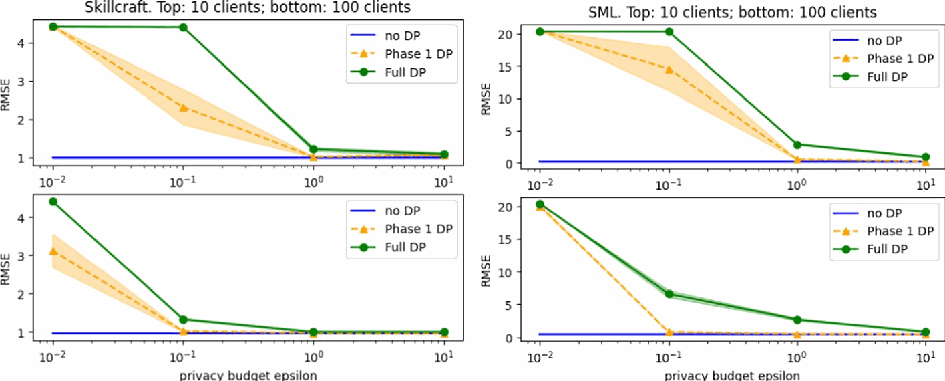
\includegraphics[width=\columnwidth]{fig_4_p18.png}
\caption{FedBNR+DP results. Left: Skillcraft dataset; right: SML dataset. Phase 1 DP: add DP protection to $\theta$ c only; full DP: add DP protection to all messages}
\label{fig:4}
\end{figure}
\section{Page 18 of 36}
Machine Learning (2026) 115:72

with them. We then discuss privacy leakage of different GP algorithms and summarize them in Table 4 . We will now discuss messages and algorithms listed in the table one by one.

Features X c or $\Phi$ c Without loss of generality, we can denote the prediction model by y = f ( $\phi$ ( x )) , where $\phi$ ( X c ) = $\Phi$ c . Then the adversaries can simply compute y c = f ( $\Phi$ c ) to recover the targets of clients. This further extends to sharing x $\star$ or $\Phi$ $\star$ , as the testing points and their corresponding targets can also be confidential.

Inducing Points U or U c There are different ways of choosing inducing points. One way is to select a subset of the training data X , and this clearly leaks raw data. Another way is to optimize them as hyperparameters. However, Smith et al. ( 2021 ) pointed out that inducing points optimized in this way often end up in regions of low data density and may corre spond to outliers. In this case, there is a high risk that some inducing points will correspond directly to real data. They proposed to use differential privacy to protect the output, but the input is left unprotected. Even in the case where inducing points lie in different spaces than the original input, it is still possible to partially recover real y c with the same argument as $\Phi$ c . Thus we want to refrain from using inducing points.

Cross Kernel Matrix k ( X c , U ) In general, sharing k ( X c , U ) does not reveal X c imme diately since the kernel function k tends to be non-invertible. However, in many algorithms that use inducing points, k ( X c , U ) serves as sufficient statistics to predict y c . For example, for FITC (Snelson \& Ghahramani, 2005 ), the predictive mean is given by:

\section{$\Lambda$ = diag [ K - k ( X , U ) k ( U , U ) - 1 k ( U , X )]}
Technique Risky message Prob lematic term

Leaked info

X c or $\Phi$ c -- -- X c , y c Inducing points U or U c -- -- $\subset$ X c k ( X c , U ) -- -- y c FedAvg ( 2017 ) N/A N/A N/A pFedGP ( 2021 ) N/A N/A N/A FedBNR (ours) N/A N/A N/A Centralized GP X c / $\Phi$ c K , k ( x $\star$ , X )

X c , y c

FITC ( 2005 ) U , k ( X c , U ) k ( X , U ) $\subset$ X c , y c pFedGP + Global Predictor U , k ( X c , U ) k ( X , U ) $\subset$ X c , y c Distributed GP ( 2015 ) x $\star$ / $\Phi$ $\star$ or X c / $\Phi$ c

k ( x $\star$ , X c ) X c , y c

or X $*$ , y $*$ Distr. Variational GPs ( 2014 ; 2016 )

U k ( U , $\cdot$ ) $\subset$ X c

SPAHM GP ( 2019 ) U k ( U , $\cdot$ ) $\subset$ X c

Risky message: messages that leak privacy but unavoidable for global prediction. Problematic term: terms that the risky messages try to compute. Leaked info: private information that can be recovered by adversaries with the risky messages. $\subset$ means ``part of''

Page 19 of 36 72

Machine Learning (2026) 115:72

Then the adversaries can again retrieve y c = k ( X c , U ) $\Sigma$ k ( U , X ) $\Lambda$ - 1 y without knowing X c .

\section{Algorithms}
FedAvg FedAvg shares no risky messages listed before. It shares model parameters only.

pFedGP Similar to FedAvg, pFedGP only shares model hyperparameters. Any prediction that requires K , k ( x $\star$ , X ) resorts to a local version K c , k ( x $\star$ , X c ) .

FedBNR In phase 1, we share hyperparameters like FedAvg and pFedGP, which is safe. In phase 2, we share hyperparameters and three other terms back and forth. No risky mes sages are shared.

$\bullet$ message 1 := $\Phi$ c $\Phi$ $^\top$ c : The outer product (known as the scatter matrix) is a non-invertible function of $\Phi$ c , and our model requires at least $\Phi$ c to predict y c . $\bullet$ message 2 := $\Phi$ c y c : This alone poses an under-constrained system of equations that has m equations and ( m + 1) n c variables, so $\Phi$ c , y c is non-identifiable. $\bullet$ message 3 := $\bar{}$ w = $\sigma$ - 2 ( $\sigma$ - 2 $\sum$

\section{c $\in$ S $\Phi$ c $\Phi$ $^\top$ c + $\lambda$ - 2 I ) - 1 $\sum$}
c $\in$ S ( $\Phi$ c y c ) : This alone poses an under-constrained system of equations that has m equations and ( m + 1) n variables, so $\Phi$ , y is non-identifiable.

In total, these three messages pose a system of equations that has m ( m + 1) / 2 + 2 m = 0 . 5 m 2 + 2 . 5 m equations and ( m + 1) n variables (i.e. $\Phi$ , y ). Since m $\ll$ n , meaning the number of random samples is much smaller than the size of training data, the system has multiple solutions and the true values of $\Phi$ , y are non-iden tifiable. Similarly, the first two messages pose a (local) system of equations that has m ( m + 1) / 2 + m = 0 . 5 m 2 + 1 . 5 m equations and ( m + 1) n c variables (i.e. $\Phi$ c , y c ). As long as 1 < m $\leq$ n c , the variables are still non-identifiable.

Centralized GP The predictive mean is given by:

f ( x $\star$ ) = k ( x $\star$ , X )( K + $\sigma$ 2 I ) - 1 y

Thus, even if we can learn the hyperparameters in a FL fashion without privacy leakage, we have to share X c / $\Phi$ c to calculate K and k ( x $\star$ , X ) .

pFedGP + Global Predictor Following the arguments with centralized GP and induc ing point approximation, pFedGP cannot generalize to a global predictor without sharing X c / $\Phi$ c (without approximation) or U and k ( X c , U ) (with the FITC approximation they adapt).

Distributed GP Deisenroth and Ng ( 2015 ) introduces a collection of works that uses the Product of Experts (PoE) model to approximate the global GP with local GPs. In the most basic setting, the global predictive mean and variance are given by:

\section{Page 20 of 36}
Machine Learning (2026) 115:72

$\mu$ ( x $\star$ ) = $\sigma$ 2 ( x $\star$ ) $\sum$

c $\in$ S $\sigma$ - 2

c ( x $\star$ ) $\mu$ c ( x $\star$ )

$\sigma$ - 2 ( x $\star$ ) =

$\sum$

c $\in$ S

$\sigma$ - 2 c ( x $\star$ )

where $\mu$ c ( x $\star$ ) and $\sigma$ 2 c ( x $\star$ ) are the local predictive mean and variance. Then, to calculate these two terms, we either have to share x $\star$ / $\Phi$ $\star$ or collect all the client experts for the tester to perform global prediction locally, where a client expert is a stand-alone GP predictive model with local training data. However, collecting client experts requires sharing X c / $\Phi$ c , by the formulas of predictive mean and variance of GP. Note all the other advanced methods proposed by Deisenroth and Ng ( 2015 ) have similar structures and thus are not safe.

Distributed Variational GPs These works are also based on inducing points, which may leak real data when clients have low data density regions, which is common for high dimen sional data.

SPAHM GP This paper did not specify technical details about the GP predictor they learned, so it remains unclear if there are other risky messages sent during the process, but they mentioned they used inducing points to learn GPs, which needs to be avoided in FL.

\section{A Differential Privacy (DP) Argument}
In this section, we show why sharing kernels is less private than sharing scatter matrices by examining how much noise is needed with DP.

The amount of noise needed with DP significantly increases when the information released has size that is dependent of the size of data, when the released information con tains non-constant interaction terms between records. This often trashes the utility of the trained model, suggesting that such messages themselves contain a lot information about the raw data and are prone to privacy bleaching. As a concrete comparison, we can calculate the sensitivity of f k ( X ) = $\Phi$( X ) $^\top$ $\Phi$( X ) , the n $\times$ n sized kernel, and f s ( X ) = $\Phi$( X )$\Phi$( X ) $^\top$ , the m $\times$ m sized scatter matrix. For simplicity, use $\Phi$( X ) = sin( X ) , $\forall$ X $\in$ R n $\times$ m so that its sensitivity is bounded. W.l.o.g, let X $'$ = X [0 : n - 1 , :] be the first n - 1 records of X . We pad f k ( X $'$ ) with 0's so that f k ( X ) and f k ( X $'$ ) are then both of size n $\times$ n . Then,

Page 21 of 36 72

Machine Learning (2026) 115:72

f k ( X ) - f k ( X $'$ ) =

k ( x 1 , x 1 ) $\cdot$ $\cdot$ $\cdot$ k ( x 1 , x n - 1 ) k ( x 1 , x n ) k ( x 2 , x 1 ) $\cdot$ $\cdot$ $\cdot$ k ( x 2 , x n - 1 ) k ( x 2 , x n ) ... ... ... ... k ( x n - 1 , x 1 ) $\cdot$ $\cdot$ $\cdot$ k ( x n - 1 , x n - 1 ) k ( x n - 1 , x n ) k ( x n , x 1 ) $\cdot$ $\cdot$ $\cdot$ k ( x n , x n - 1 ) k ( x n , x n )

-

k ( x 1 , x 1 ) $\cdot$ $\cdot$ $\cdot$ k ( x 1 , x n - 1 ) 0 k ( x 2 , x 1 ) $\cdot$ $\cdot$ $\cdot$ k ( x 2 , x n - 1 ) 0 ... ... ... ... k ( x n - 1 , x 1 ) $\cdot$ $\cdot$ $\cdot$ k ( x n - 1 , x n - 1 ) 0 0 $\cdot$ $\cdot$ $\cdot$ 0 0

=

0 $\cdot$ $\cdot$ $\cdot$ 0 k ( x 1 , x n ) 0 $\cdot$ $\cdot$ $\cdot$ 0 k ( x 2 , x n ) ... ... ... ... 0 $\cdot$ $\cdot$ $\cdot$ 0 k ( x n - 1 , x n ) k ( x n , x 1 ) $\cdot$ $\cdot$ $\cdot$ k ( x n , x n - 1 ) k ( x n , x n )

where k ( x i , x j ) = sin( x i ) $^\top$ sin( x j ) . We flatten the above matrix to a vector and cal culate the L 2 sensitivity. There are 2 n - 1 non-zero terms in the above result. Note k ( x i , x j ) $\leq$ m, $\forall$ i, j . By definition,

L 2 ( f k ) = max

X , X $'$ || flatten ( f k ( X ) - f k ( X $'$ )) || 2

= || [ 0 , $\cdot$ $\cdot$ $\cdot$ , 0 ???? ( n - 1) 2 terms

, m, $\cdot$ $\cdot$ $\cdot$ , m ? ?? ? 2 n - 1 terms

] || 2

=

$\sqrt{}$

2 n - 1 m

On the other hand, for scatter matrices,

f s ( X ) - f s ( X $'$ ) =

n ?

i =1 sin( x i ) sin( x i ) $^\top$ -

n - 1 ?

i =1 sin( x i ) sin( x i ) $^\top$

= sin( x n ) sin( x n ) $^\top$

L 2 ( f s ) = max X , X $'$ || flatten ( f s ( X ) - f s ( X $'$ )) || 2

= max x || flatten (sin( x ) sin( x ) $^\top$ ) || 2

= || [1 , $\cdot$ $\cdot$ $\cdot$ , 1 ???? m 2 terms

] || 2

= m

Since L 2 ( f k ) grows with the size of data, the magnitude of noise needed to make f k differ entially private also grows to infinity, while L 2 ( f s ) stays a small constant m $\ll$ $\sqrt{}$ 2 n - 1 m .

\section{Page 22 of 36}
Machine Learning (2026) 115:72

We acknowledge that uncertainty quantification could pose potential negative consequences for privacy. For example, it is well-known that with stationary kernels, the variance of the GP predictive posterior tends to form local minima at places where training points locate, since by definition the variance of stationary kernels depends on the distance to the training points. In this case, it is possible to at least retrieve the target y by searching for the local minima of the variance. However, this property does not hold true in general when we work with non-stationary deep kernels, where the variance depends on the input locations. Figure 5 shows an example of FedBNR where the variance adversarial attack fails. The left graph shows the ``real'' training data we wish to protect, and the corresponding predic tive posterior learned by FedBNR with a deep kernel. The right graph shows the amount of variance for the prediction in the left graph. We can see the local minima of predictive variance are reasonably far away from training data, and thus the variance adversarial attack described above fails to retrieve any training data.

To use the Gaussian mechanism to protect FedBNR, we need to add noise to all the mes sages sent by the clients. In the first phase, kernel hyperparameters are revealed. In the second phase, $\Phi$ c $\Phi$ $^\top$ c , $\Phi$ c y c , and y $^\top$ c y c are revealed. The L 2 sensitivity of each function is as follows:

$\bullet$ In phase 1, L 2 sensitivity of the hyperpameters is the L 2 gradient clipping constant times the number of local update rounds times the learning rate $\zeta$ . Since we take the average during aggregation, the actual sensitivity of the mean has an extra factor of 1 / $\sqrt{}$ n S , where n S is the number of clients. This means the more clients there are in the system, the less perturbation the mean exhibits. This factor further decreases to 1 /n S if we adapt secure multi-party computation and add noise directly to the summation of all the messages globally, instead of adding noise to messages at clients. $\bullet$ In phase 2, suppose we use the latent stationary architecture ( sin , cos activation functions normalized by $\sqrt{}$ m ), then each entry of $\Phi$ c can change by up to 2 / $\sqrt{}$ m . y is in general

Fig. 5 An example to show why variance adversarial attack fails when we have a non-stationary kernel. Left: training data and the predictive posterior of FedBNR. Right: the amount of variance for the predic tion in the left graph

Page 23 of 36 72

Machine Learning (2026) 115:72

unbounded, so we need to clip it by its max and min, and denote b := max ( y ) - min ( y ) . Then we can flatten s ( X c , y c ) = [ $\Phi$ c $\Phi$ $^\top$ c , $\Phi$ c y c , y $^\top$ c y c ] and calculate its sensitivity:

L 2 ( s ) =

$\sqrt{}$

m (2 m + 1)(4 /m ) 2 + 2 m (2 b/ $\sqrt{}$ m ) 2 + b 4 (A1)

= $\sqrt{}$

32 + 16 /m + 8 b 2 + b 4 (A2)

Note $\Phi$ c $\Phi$ $^\top$ c is symmetric and we only need to protect the upper half triangular matrix, and this architecture results in 2 m random features with m samples.

Figure 6 shows the architecture of DNNs used in the real world regression experiments. For FedAvg, FedProx, and pFedGP, we used the left DNN as their feature extractor. For our methods, we used the rightmost architecture in Fig. 2 with the same feature extractor f , a very small distribution shifter h (the right DNN in Fig. 6 ), and $\omega$ $\sim$ N ( 0 , I 5 ) .

We run each random seed of each dataset on 1 CPU and 1 NVIDIA T4 GPU with 16GB RAM. Some important hyperparameters are listed in Table 5 . These hyperparameters are selected through grid searching, as suggested by FedProx. We make our code public in the supplementary materials, where other minutiae like the learning rate can be found. All datasets included along with our code are licensed under a Creative Commons Attribution 4.0 International (CC BY 4.0) license, which allows for the sharing and adaptation of the datasets for any purpose, provided that the appropriate credit is given.

\begin{figure}[htbp]
\centering
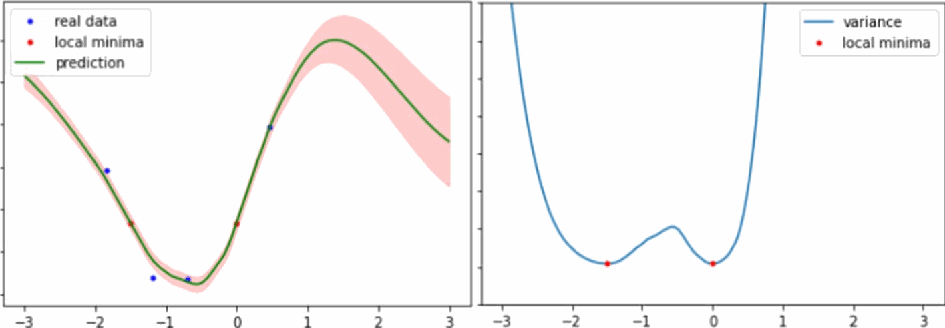
\includegraphics[width=\columnwidth]{fig_5_p23.png}
\caption{An example to show why variance adversarial attack fails when we have a non-stationary kernel. Left: training data and the predictive posterior of FedBNR. Right: the amount of variance for the predic tion in the left graph}
\label{fig:5}
\end{figure}
\section{Necessity of Random Features}
We perform an extra ablation study experiment similarly to the real-world experiment in generalization setting. Experiment details are the same as in Appendix B. Each setting is run for 10 different random seeds. RMSE reported in Table 6 shows that random features significantly improve the model capacity.

We assess models with testing data uniformly sampled globally in this setting.

We include the maximum calibration error (MCE) and the Brier score (BRI) of the real world regression experiments in Tables 7 and 8 . MCE measures the (estimated) worst differ ence between p \% confidence intervals and p $'$ \% test points falling into these intervals. BRI measures the mean squared difference between the confidence and observations, where a test point falling in the CI counts as 1, otherwise 0. We also include the standard error of the mean (SEM) in Table 9 . Our methods still perform better in most of the cases.

\section{Page 24 of 36}
Machine Learning (2026) 115:72

We report the trade-off between model utility and the privacy budget $\epsilon$ in Fig. 7 . The y-axis reports RMSE, and the light area reports the standard error of the mean (SEM). Experiments were repeated for 5 different seeds. Other experiment details are similar to the generaliza tion setting.

We assess models with testing data uniformly sampled locally in this setting.

We report MCE in Table 10 and BRI in Table 11 .

We now prove Thm. 3.1 in the main paper. We make use of the Hoeffding's inequality (Hoeffding, 1994 ).

Theorem A.1 (Hoeffding's inequality). Suppose X 1 , $\cdot$ $\cdot$ $\cdot$ , X n are n independent random variables. Let $\bar{}$ X = $\sum$ n i =1 X i /n . If $\forall$ i $\in$\{ 1 , $\cdot$ $\cdot$ $\cdot$ , n \} , Pr( X i $\in$ [ a i , b i ]) = 1 almost surely, then $\forall$ t > 0

Pr[ | $\bar{}$ X - E [ $\bar{}$ X ] | $\geq$ t ] $\leq$ 2 exp

(

- 2 t 2 n 2 $\sum$ n

i =1 ( b i - a i ) 2

)

Theorem 3.1 $\forall$ x , x $'$ $\in$ R p , $\forall$ p ( $\omega$ ) being a proper distribution over R d $'$ , and g : R d $'$ $\times$ R p -$\rightarrow$ R d has the form of Eq. 15 . With m $\in$ Z + samples of $\omega$ , $\forall$ t > 0

Pr[ | URK m $\omega$,g ( x , x $'$ ) - k ( x , x $'$ ) | $\geq$ t ] $\leq$ 2 exp

(

- mt 2

)

Proof Notice URK m $\omega$,g ( x , x $'$ ) is the empirical estimation of k ( x , x $'$ ) = E $\omega$ [ g ( $\omega$, x ) $^\top$ g ( $\omega$, x $'$ )] :

Page 25 of 36 72

Machine Learning (2026) 115:72

URK m $\omega$,g ( x , x $'$ ) =

(

s m $\omega$ ( x ) $\sqrt{}$ m

) $^\top$ (

s m $\omega$ ( x $'$ ) $\sqrt{}$ m

)

=

m $\sum$

i =1

1 m ( g ( $\omega$ i , x ) $^\top$ g ( $\omega$ i , x $'$ ))

g ( $\omega$ i , x ) $^\top$ g ( $\omega$ i , x $'$ ) are i.i.d. 1-dimensional random variables. It is bounded by [ - 2 , 2] since g ( $\omega$ , x ) = [sin( $\omega$ $^\top$ $\phi$ NN ( x )) , cos( $\omega$ $^\top$ $\phi$ NN ( x ))] $^\top$ . Finally, apply the Hoeffding's inequality. $\square$

Additionally, URK can be used to construct feature mappings of non-stationary kernels without the help of Deep Neural Networks. We prove the two examples we gave in the main paper now.

Proposition 3.2 Let $\omega$ $\sim$ N ( 0 , I ) , g ( $\omega$, x ) = exp( $\omega$ $^\top$ x ) , then k ( x , x $'$ ) = lim m -$\rightarrow$ $\infty$ URK $\omega$, g ( x , x $'$ ) has infinite features. Proof

k ( x , x $'$ ) = E $\omega$ [ z $\omega$ ( x ) $^\top$ z $\omega$ ( x $'$ )]

= E $\omega$ [exp ( $\omega$ $^\top$ ( x + x $'$ ) ) ]

= M $\omega$ ( x + x $'$ ) , the moment generating function of $\omega$

= exp(( x + x $'$ ) $^\top$ ( x + x $'$ ) / 2)

= exp(( x $^\top$ x + x $'$$^\top$ x $'$ ) / 2) exp( x $^\top$ x $'$ )

= exp(( x $^\top$ x + x $'$$^\top$ x $'$ ) / 2)

$\infty$ $\sum$

l =0

( x $^\top$ x $'$ ) l

l !

=

$\infty$ $\sum$

l =0

( exp( x $^\top$ x / 2) $\sqrt{}$

l ! ( x $^\top$ x $'$ ) l exp( x $'$$^\top$ x $'$ / 2) $\sqrt{}$

l !

)

= $\phi$ ( x ) $^\top$ $\phi$ ( x $'$ )

\section{$\square$}
Theorem 3.3 Let $\omega$ and g have the form of Prop. 3.2 . Suppose x , x $'$ $\in$ R p satisfies || x || 2 2 $\leq$ a , || x $'$ || 2 2 $\leq$ a $'$ . With m $\in$ Z + samples of $\omega$ , $\forall$ t $\in$ ( 0 , exp( a + a $'$ ) / 2 )) , by Fenton- Wilkinson approximation,

$\sigma$ s := log

( exp ( a + a $'$ ) - 1

m + 1

)

, E := exp(( a + a $'$ ) / 2)

Pr[ | URK m $\omega$,g ( x , x $'$ ) - k ( x , x $'$ ) | $\geq$ t ] $\leq$ 1 - F ( 2 log( t + E ) - ( a + a $'$ ) + $\sigma$ 2 s 2 $\sigma$ s

)

+ F

( 2 log( E - t ) - ( a + a $'$ ) + $\sigma$ 2 s 2 $\sigma$ s

)

F is the cumulative probability distribution function of the standard normal distribution.

\section{Page 26 of 36}
Machine Learning (2026) 115:72

Proof Since $\omega$ i $\sim$ N ( 0 , I ) , $\forall$ i and g ( $\omega$ i , x ) $^\top$ g ( $\omega$ i , x $'$ ) = exp( $\omega$ $^\top$ i ( x + x $'$ )) ,

$\omega$ $^\top$

i ( x + x $'$ ) $\sim$ N (0 , $\sigma$ 2 ) , $\sigma$ 2 $\leq$ a + a $'$

g ( $\omega$ i , x ) $^\top$ g ( $\omega$ i , x $'$ ) $\sim$ LogN (0 , $\sigma$ 2 ) , the log-normal distribution

Since the sum of m i.i.d. log-normal distributions has no closed form, we use the Fenton- Wilkinson approximation (Fenton, 1960 ) to model URK m $\omega$,g ( x , x $'$ ) . It approximates the sum with a log-normal distribution by matching the first and second moments.

$\sigma$ 2 s = log

( exp( $\sigma$ 2 ) - 1

m + 1

)

, E := k ( x , x $'$ ) = E [ g ( $\omega$, x ) $^\top$ g ( $\omega$, x $'$ )] = exp( $\sigma$ 2 / 2)

URK m $\omega$,g ( x , x $'$ ) =

m $\sum$

i =1

1 m ( g ( $\omega$ i , x ) $^\top$ g ( $\omega$ i , x $'$ )) $\sim$ LogN (( $\sigma$ 2 - $\sigma$ 2 s ) / 2 , $\sigma$ 2 s )

Pr[ URK m $\omega$,g ( x , x $'$ ) - E $\geq$ t ] = 1 - Pr[ URK m $\omega$,g ( x , x $'$ ) $\leq$ t + E ]

\section{= 1 - F ( 2 log( t + E ) - $\sigma$ 2 + $\sigma$ 2 s 2 $\sigma$ s}
)

Pr[ URK m $\omega$,g ( x , x $'$ ) - E $\leq$- t ] = Pr[ URK m $\omega$,g ( x , x $'$ ) $\leq$ E - t ]

\section{= F ( 2 log( E - t ) - $\sigma$ 2 + $\sigma$ 2 s 2 $\sigma$ s}
)

Pr[ | URK m

$\omega$,g ( x , x $'$ ) - k ( x , x $'$ ) | $\geq$ t ] = Pr[ URK m

$\omega$,g ( x , x $'$ ) - E $\geq$ t ] + Pr[ URK m

$\omega$,g ( x , x $'$ ) - E $\leq$- t ]

This equation takes its maximum when $\sigma$ 2 = a + a $'$ . $\square$

\section{Proposition 3.4 Let $\tilde{}$c , $\tilde{}$n $\in$ R . Define $\tilde{}$ p = [ 1}
2 , 1 2p , 1 2p , $\cdot$ $\cdot$ $\cdot$ , 1 2p ] $^\top$ $\in$ R p + 1 , $\omega$ $\sim$ Multi ( $\tilde{}$n , $\tilde{}$ p ) , the multino mial distribution. Define $\tilde{}$ x = [ $\sqrt{}$

2$\tilde{}$c , $\sqrt{}$ 2p x $^\top$ ] $^\top$ $\in$ R p + 1 , g ( $\omega$, x ) = exp( $\omega$ $^\top$ log $\tilde{}$ x ) , then k ( x , x $'$ ) = lim m -$\rightarrow$ $\infty$ URK $\omega$, g ( x , x $'$ ) = ( x $^\top$ x $'$ + $\tilde{}$c ) $\tilde{}$n

Proof In the following proof, any subscript i means the i th entry of the vector. By definition,

k ( x , x $'$ ) = E $\omega$ [ z $\omega$ ( x ) $^\top$ z $\omega$ ( x $'$ )]

= E $\omega$ [exp ( $\omega$ $^\top$ (log $\tilde{}$ x + log $\tilde{}$ x $'$ ) ) ]

= M $\omega$ (log $\tilde{}$ x + log $\tilde{}$ x $'$ ) , the moment generating function of $\omega$

=

( p +1 $\sum$

i =1 p poly,i exp(log $\tilde{}$ x i + log $\tilde{}$ x $'$ i )

) $\tilde{}$ n

=

( 1 2 exp(2 log $\sqrt{}$

2$\tilde{}$ c ) +

p $\sum$

i =1

1 2 p exp(log $\sqrt{}$

2 p x i + log $\sqrt{}$

2 p x $'$ i )

) $\tilde{}$ n

=

(

$\tilde{}$ c +

p $\sum$

i =1 x i x $'$ i

) $\tilde{}$ n

= ( x $^\top$ x $'$ + $\tilde{}$ c ) $\tilde{}$ n

Page 27 of 36 72

Machine Learning (2026) 115:72

\section{$\square$}
Theorem 3.5 Let $\omega$ and g have the form of Prop. 3.4 . Suppose entries of x , x $'$ $\in$ R p + are bounded by [a, b]. With m $\in$ Z + samples of $\omega$ , $\forall$ t > 0 ,

v := max \{

$\sqrt{}$

2$\tilde{}$ c, $\sqrt{}$ 2 pb \} min \{ $\sqrt{}$

2$\tilde{}$ c, $\sqrt{}$ 2 pa \}

Pr[ | URK m $\omega$,g ( x , x $'$ ) - k ( x , x $'$ ) | $\geq$ t ] $\leq$ 2 exp

( - 2 mt 2

v 4$\tilde{}$ n

)

Proof Similarly to Thm. 2, g ( $\omega$ i , x ) $^\top$ g ( $\omega$ i , x $'$ ) are i.i.d. 1-dimensional random variables, bounded by [exp($\tilde{}$ n log( min \{ $\sqrt{}$

2$\tilde{}$ c, $\sqrt{}$ 2 pa \} )) , exp($\tilde{}$ n log( max \{ $\sqrt{}$

2$\tilde{}$ c, $\sqrt{}$ 2 pb \} ))] . Then, apply Hoeffding's inequality. $\square$

Fig. 6 Architecture of DNNs used in real world regression experiments. Left: the feature extractor for x ; right: the distribution shifter for $\omega$ . FC is short for ``fully connected''. The layer size s varies for different datasets

\section{Page 28 of 36}
Machine Learning (2026) 115:72

Page 29 of 36 72

Machine Learning (2026) 115:72

\#Clients Skillcraft SML Parkinsons Bike CCPP

\begin{figure}[htbp]
\centering
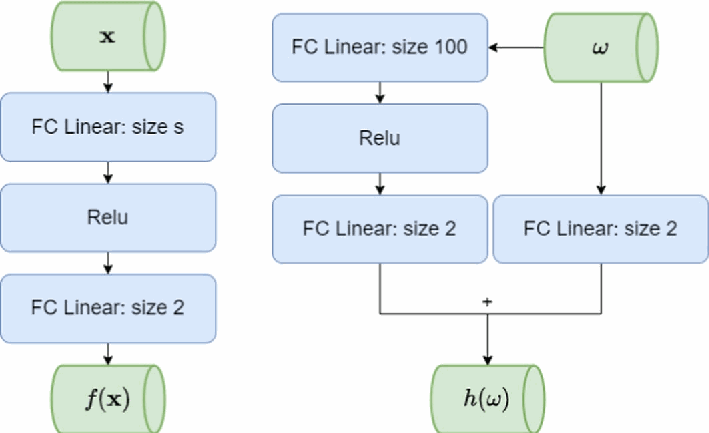
\includegraphics[width=\columnwidth]{fig_6_p28.png}
\caption{Architecture of DNNs used in real world regression experiments. Left: the feature extractor for x ; right: the distribution shifter for $\omega$ . FC is short for ``fully connected''. The layer size s varies for different datasets}
\label{fig:6}
\end{figure}
\section{Page 30 of 36}
Machine Learning (2026) 115:72

Fig. 7 FedBNR+DP results. Phase 1 DP: add DP protection to model parameters $\theta$ only; full DP: add DP protection to all messages

Page 31 of 36 72

Machine Learning (2026) 115:72

Supplementary Information The online version contains supplementary material available at https://doi.org /10.1007/s10994-025-06936-5 .

Acknowledgements Resources used in preparing this research at the University of Waterloo were provided by Huawei Canada, the province of Ontario and the government of Canada through CIFAR and companies sponsoring the Vector Institute.

Author Contributions H.Y., K.G., M.K., G.Z., and P.P. contributed to the study conception and design. Mate rial preparation, data collection and analysis were performed by H.Y. The first draft of the manuscript was written by H.Y. and P.P. All authors commented on previous versions of the manuscript. All authors read and approved the final manuscript.

Funding The research leading to these results received funding from Huawei Canada under Grant Agreement \#TC20210831001 and the AI Chair program of the Canadian Institute for Advanced Research (CIFAR).

Data Availability No datasets were generated or analysed during the current study.

Materials Availability Not applicable.

Code Availability We provide public code in the supplementary file.

\begin{figure}[htbp]
\centering
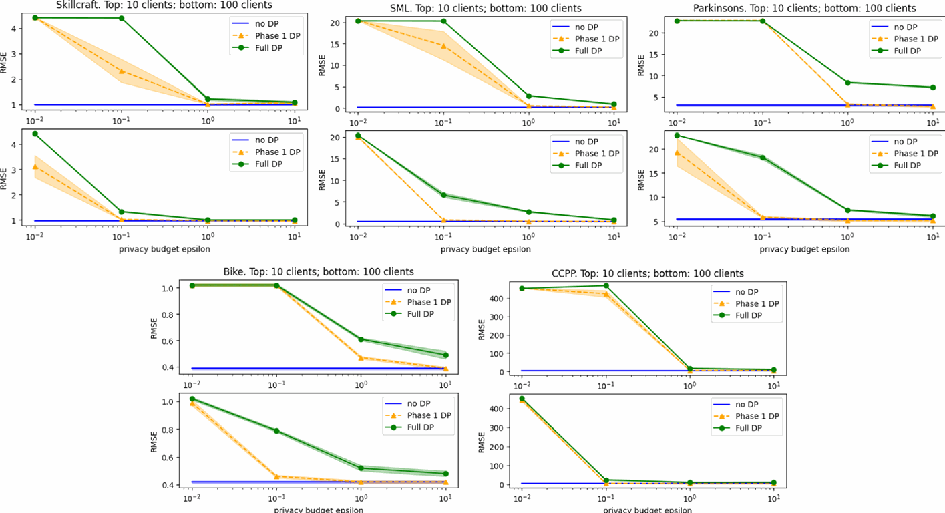
\includegraphics[width=\columnwidth]{fig_7_p31.png}
\caption{FedBNR+DP results. Phase 1 DP: add DP protection to model parameters $\theta$ only; full DP: add DP protection to all messages}
\label{fig:7}
\end{figure}
\section{Declarations}
Conflict of interest The authors declare no Conflict of interest.

Ethical Approval Not applicable.

Consent to Participate Not applicable.

Consent for Publication All authors consent to the submission of this manuscript to the Machine Learning .

\begin{thebibliography}{99}
\bibitem{ref1} Achituve, I., Shamsian, A., Navon, A., Chechik, G., \& Fetaya, E. (2021). Personalized federated learning with Gaussian processes. Advances in Neural Information Processing Systems, 34 , 8392--8406. Begoli, E., Bhattacharya, T., \& Kusnezov, D. (2019). The need for uncertainty quantification in machine- assisted medical decision making. Nature Machine Intelligence, 1 (1), 20--23. Boenisch, F., Dziedzic, A., Schuster, R., Shamsabadi, A. S., Shumailov, I., \& Papernot, N. (2021). When the curious abandon honesty: Federated learning is not private . arXiv preprint arXiv:2112.02918 . Byrd, D., \& Polychroniadou, A. (2020). Differentially private secure multi-party computation for federated learning in financial applications. In: Proceedings of the first ACM international conference on AI in Finance , pp. 1--9. Calandra, R., Peters, J., Rasmussen, C. E., \& Deisenroth, M. P. (2016). Manifold Gaussian processes for regression. In: 2016 International joint conference on neural networks (IJCNN) , pp. 3338--3345. IEEE. Cao, Y., \& Fleet, D. J. (2014). Generalized product of experts for automatic and principled fusion of Gauss ian process predictions . arXiv preprint arXiv:1410.7827 . Cuturi, M. (2009). Positive definite kernels in machine learning . arXiv preprint arXiv:0911.5367 . Damianou, A., \& Lawrence, N.D. (2013). Deep gaussian processes. In: Artificial intelligence and statistics , pp. 207--215. PMLR. Danquah, B., Riedmaier, S., Rühm, J., Kalt, S., \& Lienkamp, M. (2020). Statistical model verification and validation concept in automotive vehicle design. Procedia Cirp, 91 , 261--270. Deisenroth, M., \& Ng, J.W. (2015). Distributed gaussian processes. In: International conference on machine learning , pp. 1481--1490. PMLR.
\bibitem{ref2} Fenton, L. (1960). The sum of log-normal probability distributions in scatter transmission systems. IRE
\bibitem{ref3} Transactions on Communications Systems, 8 (1), 57--67. Gal, Y., \& Ghahramani, Z. (2016). Dropout as a Bayesian approximation: Representing model uncertainty in deep learning. In: International Conference on Machine Learning , pp. 1050--1059. PMLR. Gal, Y., Van Der Wilk, M., \& Rasmussen, C. E. (2014). Distributed variational inference in sparse Gaussian process regression and latent variable models. Advances in Neural Information Processing Systems , 27 . Garnelo, M., Rosenbaum, D., Maddison, C., Ramalho, T., Saxton, D., Shanahan, M., Teh, Y. W., Rezende, D., \& Eslami, S.A. (2018). Conditional neural processes. In: International conference on machine learning , pp. 1704--1713. PMLR. Gawlikowski, J., Tassi, C. R. N., Ali, M., Lee, J., Humt, M., Feng, J., Kruspe, A., Triebel, R., Jung, P.,
\bibitem{ref4} Roscher, R., Shahzad, M., Yang, W., Bamler, R., \& Zhu, X. X. (2022). A survey of uncertainty in deep neural networks . He, B., \& Ozay, M. (2022). Feature kernel distillation. In: International conference on learning representations . He, K., Zhang, X., Ren, S., \& Sun, J. (2016). Deep residual learning for image recognition. In: Proceedings of the IEEE conference on computer vision and pattern recognition , pp. 770--778. Hensman, J., Fusi, N., \& Lawrence, N. D. (2013). Gaussian processes for big data . arXiv preprint arXiv:1309.6835 . Hinton, G. E., \& Salakhutdinov, R. R. (2007). Using deep belief nets to learn covariance kernels for Gaussian processes. Advances in Neural Information Processing Systems , 20 . Hoang, T. N., Hoang, Q. M., \& Low, B. K. H. (2016). A distributed variational inference framework for unifying parallel sparse Gaussian process regression models. In: International conference on machine learning , pp. 382--391. PMLR. Hoeffding, W. (1994). Probability inequalities for sums of bounded random variables . The collected works of Wassily Hoeffding, 409--426. Iyer, A., Zhang, Y., Prasad, A., Gupta, P., Tao, S., Wang, Y., Prabhune, P., Schadler, L. S., Brinson, L. C., \& Chen, W. (2020). Data centric nanocomposites design via mixed-variable Bayesian optimization. Molecular Systems Design \& Engineering, 5 (8), 1376--1390. Iyer, A., Zhang, Y., Prasad, A., Tao, S., Wang, Y., Schadler, L., Brinson, L. C., \& Chen, W. (2019). Data- centric mixed-variable Bayesian optimization for materials design. In: International design engineer ing technical conferences and computers and information in engineering conference , vol. 59186, pp. 02--03066. American Society of Mechanical Engineers. Karimireddy, S. P., Kale, S., Mohri, M., Reddi, S., Stich, S., \& Suresh, A. T. (2020). Scaffold: Stochas tic controlled averaging for federated learning. In: International conference on machine learning , pp. 5132--5143. PMLR Kerkouche, R., Ács, G., Castelluccia, C., \& Genevès, P. (2021). Privacy-preserving and bandwidth-efficient ing: Strategies for improving communication efficiency . arXiv preprint arXiv:1610.05492 . Kontoudis, G. P., \& Stilwell, D. J. (2023). Decentralized federated learning using gaussian processes. In: 2023 International symposium on multi-robot and multi-agent systems (MRS) , pp. 1--7. IEEE. Kontoudis, G. P., \& Stilwell, D. J. (2024). Scalable, federated gaussian process training for decentralized multi-agent systems. IEEE Access, 12 , 77800--77815. Kristiadi, A., Hein, M., \& Hennig, P. (2020). Being Bayesian, even just a bit, fixes overconfidence in ReLU networks . Lederer, A., Umlauft, J., \& Hirche, S. (2019). Uniform error bounds for gaussian process regression with application to safe control. Advances in Neural Information Processing Systems , 32 . Li, T., Sahu, A. K., Zaheer, M., Sanjabi, M., Talwalkar, A., \& Smith, V. (2020). Federated optimization in heterogeneous networks. Proceedings of Machine Learning and Systems, 2 , 429--450. Li, Y., Rao, S., Hassaine, A., Ramakrishnan, R., Canoy, D., Salimi-Khorshidi, G., Mamouei, M., Lukasie wicz, T., \& Rahimi, K. (2021). Deep Bayesian gaussian processes for uncertainty estimation in elec tronic health records. Scientific Reports, 11 (1), 20685. Li, Y., Zhou, Y., Jolfaei, A., Yu, D., Xu, G., \& Zheng, X. (2020). Privacy-preserving federated learning frame work based on chained secure multiparty computing. IEEE Internet of Things Journal, 8 (8), 6178--6186. Liu, H., Ong, Y.-S., Shen, X., \& Cai, J. (2020). When Gaussian process meets big data: A review of scalable gps. IEEE Transactions on Neural Networks and Learning Systems, 31 (11), 4405--4423. McMahan, B., Moore, E., Ramage, D., Hampson, S., \& Arcas, B. A. (2017). Communication-efficient learn ing of deep networks from decentralized data. In: Artificial intelligence and statistics , pp. 1273--1282. PMLR.
\bibitem{ref5} Mohri, M., Sivek, G., \& Suresh, A. T. (2019). Agnostic federated learning. In: International conference on machine learning , pp. 4615--4625. PMLR. Mothukuri, V., Parizi, R. M., Pouriyeh, S., Huang, Y., Dehghantanha, A., \& Srivastava, G. (2021). A survey on security and privacy of federated learning. Future Generation Computer Systems, 115 , 619--640. Nickson, T., Gunter, T., Lloyd, C., Osborne, M. A., \& Roberts, S. (2015). Blitzkriging: Kronecker-structured stochastic Gaussian processes . arXiv preprint arXiv:1510.07965 . Ober, S. W., Rasmussen, C. E., \& Wilk, M. (2021). The promises and pitfalls of deep kernel learning. In:
\bibitem{ref6} Uncertainty in artificial intelligence , pp. 1206--1216. PMLR. Oliva, J. B., Dubey, A., Wilson, A. G., Póczos, B., Schneider, J., \& Xing, E. P. (2016). Bayesian nonparamet ric kernel-learning. In: Artificial intelligence and statistics , pp. 1078--1086. PMLR. Quinonero-Candela, J., \& Rasmussen, C. E. (2005). A unifying view of sparse approximate Gaussian process regression. The Journal of Machine Learning Research, 6 , 1939--1959. Rahimi, A., \& Recht, B. (2007). Random features for large-scale kernel machines. Advances in Neural Infor mation Processing Systems , 20 . Reisizadeh, A., Mokhtari, A., Hassani, H., Jadbabaie, A., \& Pedarsani, R. (2020). Fedpaq: A communication- efficient federated learning method with periodic averaging and quantization. In: International confer ence on artificial intelligence and statistics , pp. 2021--2031. PMLR. Riedmaier, S., Danquah, B., Schick, B., \& Diermeyer, F. (2021). Unified framework and survey for model verification, validation and uncertainty quantification. Archives of Computational Methods in Engineer ing, 28 , 2655--2688. Riedmaier, S., Ponn, T., Ludwig, D., Schick, B., \& Diermeyer, F. (2020). Survey on scenario-based safety assessment of automated vehicles. IEEE Access, 8 , 87456--87477. Rudin, W. (2017). Fourier analysis on groups . Garden City: Courier Dover Publications. Saatçi, Y. (2012). Scalable inference for structured Gaussian process models . PhD thesis, Citeseer. Sattler, F., Wiedemann, S., Müller, K.-R., \& Samek, W. (2019). Robust and communication-efficient feder ated learning from non-iid data. IEEE Transactions on Neural Networks and Learning Systems, 31 (9), 3400--3413. Schwaighofer, A., \& Tresp, V. (2002). Transductive and inductive methods for approximate Gaussian process regression. Advances in Neural Information Processing Systems , 15 . Seeger, M. W., Williams, C. K., \& Lawrence, N. D. (2003). Fast forward selection to speed up sparse Gauss ian process regression. In: International workshop on artificial intelligence and statistics , pp. 254--261. PMLR. Shoham, N., Avidor, T., Keren, A., Israel, N., Benditkis, D., Mor-Yosef, L., \& Zeitak, I. (2019). Overcoming forgetting in federated learning on non-iid data . arXiv preprint arXiv:1910.07796 . Sinha, A., \& Duchi, J. C. (2016). Learning kernels with random features. Advances in Neural Information
\bibitem{ref7} Processing Systems , 29 . Smith, M. T., Álvarez, M. A., \& Lawrence, N. D. (2021). Differentially private regression and classification with sparse Gaussian processes. Journal of Machine Learning Research, 22 , 188. Smola, A., \& Bartlett, P. (2000). Sparse greedy Gaussian process regression. Advances in Neural Information
\bibitem{ref8} Processing Systems , 13 . Snelson, E., \& Ghahramani, Z. (2005). Sparse Gaussian processes using pseudo-inputs. Advances in Neural
\bibitem{ref9} Information Processing Systems , 18 . Tang, M., Ning, X., Wang, Y., Wang, Y., \& Chen, Y. (2021). Fedgp: Correlation-based active client selection strategy for heterogeneous federated learning . arXiv preprint arXiv:2103.13822 . Thompson, J. J., Blair, M. R., Chen, L., \& Henrey, A. J. (2013). Video game telemetry as a critical tool in the study of complex skill learning. PLoS ONE, 8 (9), 75129. Titsias, M. (2009). Variational learning of inducing variables in sparse Gaussian processes. In: Artificial intel ligence and statistics , pp. 567--574. PMLR. Tran, G.-L., Bonilla, E. V., Cunningham, J., Michiardi, P., \& Filippone, M. (2019). Calibrating deep convolu tional Gaussian processes. In: The 22nd international conference on artificial intelligence and statistics , pp. 1554--1563. PMLR. Triastcyn, A., \& Faltings, B. (2019). Federated learning with bayesian differential privacy. In: 2019 IEEE international conference on big data (Big Data) , pp. 2587--2596. IEEE. Truex, S., Baracaldo, N., Anwar, A., Steinke, T., Ludwig, H., Zhang, R., \& Zhou, Y. (2019). A hybrid approach to privacy-preserving federated learning. In: Proceedings of the 12th ACM workshop on artificial intel ligence and security , pp. 1--11. Tsanas, A., Little, M., McSharry, P., \& Ramig, L. (2009). Accurate telemonitoring of Parkinson's disease progression by non-invasive speech tests. Nature Proceedings pp. 1--1. Tüfekci, P. (2014). Prediction of full load electrical power output of a base load operated combined cycle power plant using machine learning methods. International Journal of Electrical Power \& Energy Systems, 60 , 126--140.
\bibitem{ref10} Ve, S., \& Cho, Y. (2020). A rule-based model for Seoul bike sharing demand prediction using weather data.
\bibitem{ref11} European Journal of Remote Sensing, 53 (sup1), 166--183. Verrelst, J., Rivera, J. P., Moreno, J., \& Camps-Valls, G. (2013). Gaussian processes uncertainty estimates in experimental sentinel-2 lai and leaf chlorophyll content retrieval. ISPRS Journal of Photogrammetry and Remote Sensing, 86 , 157--167. Wei, K., Li, J., Ding, M., Ma, C., Yang, H. H., Farokhi, F., Jin, S., Quek, T. Q., \& Poor, H. V. (2020). Feder ated learning with differential privacy: Algorithms and performance analysis. IEEE Transactions on Information Forensics and Security, 15 , 3454--3469. Wilcoxon, F. (1992). Individual comparisons by ranking methods. In: Breakthroughs in statistics , pp. 196-- 202. Springer. Wilson, A. G., Dann, C., \& Nickisch, H. (2015). Thoughts on massively scalable Gaussian processes . arXiv preprint arXiv:1511.01870 . Wilson, A. G., Hu, Z., Salakhutdinov, R. R., \& Xing, E. P. (2016a). Stochastic variational deep kernel learn ing. Advances in Neural Information Processing Systems, 29 , 2586--2594. Wilson, A. G., Hu, Z., Salakhutdinov, R., \& Xing, E. P. (2016b). Deep kernel learning. In: Artificial intel ligence and statistics , pp. 370--378. PMLR. Wilson, A., \& Nickisch, H. (2015). Kernel interpolation for scalable structured Gaussian processes (kiss-gp). In: International conference on machine learning , pp. 1775--1784. PMLR. Xia, X., Sivonxay, E., Helms, B. A., Blau, S. M., \& Chan, E. M. (2023). Accelerating the design of multishell upconverting nanoparticles through Bayesian optimization. Nano Letters, 23 (23), 11129--11136. Xie, A., Yin, F., Xu, Y., Ai, B., Chen, T., \& Cui, S. (2019). Distributed Gaussian processes hyperparameter optimization for big data using proximal admm. IEEE Signal Processing Letters, 26 (8), 1197--1201. Yin, F., Lin, Z., Kong, Q., Xu, Y., Li, D., Theodoridis, S., \& Cui, S. R. (2020). Fedloc: Federated learning framework for data-driven cooperative localization and location data processing. IEEE Open Journal of Signal Processing, 1 , 187--215. Yurochkin, M., Agarwal, M., Ghosh, S., Greenewald, K., \& Hoang, N. (2019). Statistical model aggregation via parameter matching. Advances in Neural Information Processing Systems , 32 . Zamora-Martinez, F., Romeu, P., Botella-Rocamora, P., \& Pardo, J. (2014). On-line learning of indoor tem perature forecasting models towards energy efficiency. Energy and Buildings, 83 , 162--172. Zhu, H., Xu, J., Liu, S., \& Jin, Y. (2021). Federated learning on non-iid data: A survey. Neurocomputing, 465 , 371--390.
\end{thebibliography}
\end{document}